\documentclass[11pt,a4paper]{report}
\usepackage[utf8]{inputenc}
\usepackage[T1]{fontenc}
\usepackage{amsmath}
\usepackage{amsfonts}
\usepackage{amssymb}
\usepackage{graphicx}

\graphicspath{ {fig/} }

\usepackage{color}
\usepackage{tabularx}
\usepackage{pdfpages}
\usepackage{float}
\usepackage{listings}
\usepackage[left=2.5cm,top=2cm,right=2.5cm,bottom=2cm,bindingoffset=0.5cm]{geometry}
\usepackage{subcaption}

\usepackage{rotating}
\usepackage[font={small,it}]{caption}

\usepackage[backend=bibtex8]{biblatex}
\bibliography{/Users/tobiasstal/proj/ref/ref.bib}

\usepackage{advdate}

\usepackage{xcolor}
\usepackage{mdframed}

\usepackage{titling}

\pretitle{\begin{center}\Huge\bfseries}
	\posttitle{\par\end{center}\vskip 0.5em}
\preauthor{\begin{center}\Large\ttfamily}
	\postauthor{\end{center}}
\predate{\par\large\centering}
\postdate{\par}

\author{Tobias Staal}
\title{Spatial Baysean Changepoint Detection\\ - \\ Progress Report 2}
\date{\AdvanceDate[-1]\today}
\begin{document}

	
	
\def \NaiveFile {NOOOO}\def \NaiveFile {NOOOO}\def \NaiveFile {NOOOO}\def \NaiveFile {NOOOO}\def \Conclusion {\textcolor{red}{(No data)}}\def \NaiveFile {NOOOO}\def \Conclusion {\textcolor{red}{(No data)}}\def \NaiveFile {NOOOO}\def \conclusion {\textcolor{red}{(No data)}}\def \NaiveFile {ga_vpt_line_2}\def \conclusion {\textcolor{red}{(No data) }}\def \NaiveFile {ga_vpt_line_2}\def \conclusion {\textcolor{red}{(No data) }}\def \NaiveFile {ga_vpt_line_2} 
\def \conclusion {\textcolor{red}{(No data) }} 
\def \NaiveFile {ga_vpt_line_2} 
\def \conclusion {\textcolor{red}{(No data) }} 
\def \NaiveFile {ga_vpt_line_2} 
\def \conclusion {\textcolor{red}{(No data) }} 
\def \NaiveFile {ga_vpt_line_2} 
\def \conclusion {\textcolor{red}{(No data) }} 
\def \NaiveFile {ga_vpt_line_2} 
\def \conclusion {\textcolor{red}{(No data) }} 
\def \NaiveFile {ga_vpt_line_2} 
\def \conclusion {\textcolor{red}{(No data) }} 
\def \NaiveFile {ga_vpt_line_2} 
\def \conclusion {\textcolor{red}{(No data) }} 
\def \NaiveFile {ga_vpt_line_2} 
\def \conclusion {\textcolor{red}{(No data) }} 
\def \NaiveFile {ga_vpt_line_2} 
\def \conclusion {\textcolor{red}{(No data) }} 
\def \NaiveFile {ga_vpt_line_2} 
\def \conclusion {\textcolor{red}{(No data) }} 
\def \NaiveFile {ga_vpt_line_2} 
\def \conclusion {\textcolor{red}{(No data) }} 
\def \NaiveFile {ga_vpt_line_2} 
\def \conclusion {\textcolor{red}{(No data) }} 
\def \NaiveFile {ga_vpt_line_2} 
\def \conclusion {\textcolor{red}{(No data) }} 
\def \NaiveFile {ga_vpt_line_2} 
\def \conclusion {\textcolor{red}{(No data) }} 
\def \NaiveFile {ga_vpt_line_2} 
\def \conclusion {\textcolor{red}{(No data) }} 
\def \NaiveFile {ga_vpt_line_2} 
\def \conclusion {\textcolor{red}{(No data) }} 
\def \NaiveFile {ga_vpt_line_2} 
\def \conclusion {\textcolor{red}{(No data) }} 
\def \NaiveFile {ga_vpt_line_2} 
\def \conclusion {\textcolor{red}{(No data) }} 
\def \NaiveFile {ga_vpt_line_2} 
\def \conclusion {\textcolor{red}{(No data) }} 
\def \NaiveFile {ga_vpt_line_2} 
\def \conclusion {\textcolor{red}{(No data) }} 
\def \NaiveFile {ga_vpt_line_2} 
\def \conclusion {\textcolor{red}{(No data) }} 
\def \NaiveFile {ga_vpt_line_2} 
\def \conclusion {\textcolor{red}{(No data) }} 
\def \NaiveFile {ga_vpt_line_2} 
\def \conclusion {\textcolor{red}{(No data) }} 
\def \NaiveFile {ga_vpt_line_2} 
\def \conclusion {\textcolor{red}{(No data) }} 
\def \NaiveFile {ga_vpt_line_2} 
\def \conclusion {\textcolor{red}{(No data) }} 
\def \NaiveFile {ga_vpt_line_2} 
\def \conclusion {\textcolor{red}{(No data) }} 
\def \NaiveFile {ga_vpt_line_2} 
\def \conclusion {\textcolor{red}{(No data) }} 
\def \NaiveFile {ga_vpt_line_2} 
\def \conclusion {\textcolor{red}{(No data) }} 
\def \NaiveFile {ga_vpt_line_2} 
\def \conclusion {\textcolor{red}{(No data) }} 
\def \NaiveFile {ga_vpt_line_2} 
\def \conclusion {\textcolor{red}{(No data) }} 
\def \NaiveFile {ga_vpt_line_2} 
\def \conclusion {\textcolor{red}{(No data) }} 
\def \NaiveFile {ga_vpt_line_2} 
\def \conclusion {\textcolor{red}{(No data) }} 
\def \NaiveFile {ga_vpt_line_2} 
\def \conclusion {\textcolor{red}{(No data) }} 
\def \NaiveFile {ga_vpt_line_2} 
\def \conclusion {\textcolor{red}{(No data) }} 
\def \NaiveFile {ga_vpt_line_2} 
\def \conclusion {\textcolor{red}{(No data) }} 
\def \NaiveFile {ga_vpt_line_2} 
\def \conclusion {\textcolor{red}{(No data) }} 
\def \NaiveFile {ga_vpt_line_2} 
\def \conclusion {\textcolor{red}{(No data) }} 
\def \NaiveFile {ga_vpt_line_2} 
\def \conclusion {\textcolor{red}{(No data) }} 
\def \NaiveFile {ga_vpt_line_2} 
\def \conclusion {\textcolor{red}{(No data) }} 
\def \NaiveFile {ga_vpt_line_2} 
\def \conclusion {\textcolor{red}{(No data) }} 
\def \NaiveFile {ga_vpt_line_2} 
\def \conclusion {\textcolor{red}{(No data) }} 
\def \NaiveFile {ga_vpt_line_2} 
\def \conclusion {\textcolor{red}{(No data) }} 
\def \NaiveFile {ga_vpt_line_2} 
\def \conclusion {\textcolor{red}{(No data) }} 
\def \NaiveFile {ga_vpt_line_2} 
\def \conclusion {\textcolor{red}{(No data) }} 
\def \NaiveFile {ga_vpt_line_2} 
\def \conclusion {\textcolor{red}{(No data) }} 
\def \NaiveFile {ga_vpt_line_2} 
\def \conclusion {\textcolor{red}{(No data) }} 
\def \NaiveFile {ga_vpt_line_2} 
\def \conclusion {\textcolor{red}{(No data) }} 
\def \NaiveFile {ga_vpt_line_2} 
\def \conclusion {\textcolor{red}{(No data) }} 
\def \NaiveFile {ga_vpt_line_2} 
\def \conclusion {\textcolor{red}{(No data) }} 
\def \NaiveFile {ga_vpt_line_2} 
\def \conclusion {\textcolor{red}{(No data) }} 
\def \NaiveFile {ga_vpt_line_2} 
\def \conclusion {\textcolor{red}{(No data) }} 
\def \NaiveFile {ga_vpt_line_2} 
\def \conclusion {\textcolor{red}{(No data) }} 
\def \NaiveFile {ga_vpt_line_2} 
\def \conclusion {\textcolor{red}{(No data) }} 
\def \NaiveFile {ga_vpt_line_2} 
\def \conclusion {\textcolor{red}{(No data) }} 
\def \NaiveFile {ga_vpt_line_2} 
\def \conclusion {\textcolor{red}{(No data) }} 
\def \NaiveFile {ga_vpt_line_2} 
\def \conclusion {\textcolor{red}{(No data) }} 
\def \NaiveFile {ga_vpt_line_2} 
\def \conclusion {\textcolor{red}{(No data) }} 
\def \NaiveFile {ga_vpt_line_2} 
\def \conclusion {\textcolor{red}{(No data) }} 
\def \NaiveFile {ga_vpt_line_2} 
\def \conclusion {\textcolor{red}{(No data) }} 
\def \NaiveFile {ga_vpt_line_2} 
\def \conclusion {\textcolor{red}{(No data) }} 
\def \NaiveFile {ga_vpt_line_2} 
\def \conclusion {\textcolor{red}{(No data) }} 
\def \NaiveFile {ga_vpt_line_2} 
\def \conclusion {\textcolor{red}{(No data) }} 
\def \NaiveFile {ga_vpt_line_2} 
\def \conclusion {\textcolor{red}{(No data) }} 
\def \NaiveFile {ga_vpt_line_2} 
\def \conclusion {\textcolor{red}{(No data) }} 
\def \NaiveFile {ga_vpt_line_2} 
\def \conclusion {\textcolor{red}{(No data) }} 
\def \NaiveFile {ga_vpt_line_2} 
\def \conclusion {\textcolor{red}{(No data) }} 
\def \conclusion {\textcolor{red}{(No data) }} 
\def \conclusion {\textcolor{red}{(No data) }} 
\def \conclusion {\textcolor{red}{(No data) }} 
\def \conclusion {\textcolor{red}{(No data) }} 
\def \conclusion {\textcolor{red}{(No data) }} 
\def \conclusion {\textcolor{red}{(No data) }} 
\def \conclusion {\textcolor{red}{(No data) }} 
\def \conclusion {\textcolor{red}{(No data) }} 
\def \conclusion {\textcolor{red}{(No data) }} 
\def \conclusion {\textcolor{red}{(No data) }} 
\def \conclusion {\textcolor{red}{(No data) }} 
\def \conclusion {\textcolor{red}{(No data) }} 
\def \conclusion {\textcolor{red}{(No data) }} 
\def \conclusion {\textcolor{red}{(No data) }} 
\def \conclusion {\textcolor{red}{(No data) }} 
\def \conclusion {\textcolor{red}{(No data) }} 
\def \conclusion {\textcolor{red}{(No data) }} 
\def \conclusion {\textcolor{red}{(No data) }} 
\def \conclusion {\textcolor{red}{(No data) }} 
\def \conclusion {\textcolor{red}{(No data) }} 
\def \conclusion {\textcolor{red}{(No data) }} 
\def \conclusion {\textcolor{red}{(No data) }} 
\def \conclusion {\textcolor{red}{(No data) }} 
\def \conclusion {\textcolor{red}{(No data) }} 
\def \conclusion {\textcolor{red}{(No data) }} 
\def \conclusion {\textcolor{red}{(No data) }} 
\def \conclusion {\textcolor{red}{(No data) }} 
\def \conclusion {\textcolor{red}{(No data) }} 
\def \conclusion {\textcolor{red}{(No data) }} 


\maketitle




%1 - Focus on a smaller number of lines to start with, please do…  
%Line 12 (across Pilbara/Capricorn to Yilgarn, terranes well defined and some surface exposure)
%Line 2 (orogens, comparision with Line 12, terranes mostly undercover)

%Could you focus the getting the initial multivariable changepoint code going on these lines?   When you have some results we will have a skype meeting.  Happy to look at other lines also, but these ones will be most telling in the first instance.  

%a) Point of review, assuming you are working on this most of the time, 19 March - Tobias to send short e-mail update to all whether things are working or not.

%b) Pre-skype meeting, send .pdf for discussion. Include 7 March results on line 12 also because these univariate results will be quite informative alongside the multivariate.  Note that there are some statistical inference ideas that we should discuss also.  We will exchange e-mails before the Skype meeting on data used, preprocessing, results, best interpretation, application to Antarctica (amongst other things).

%2 - Tobias to write a research schedule (an ordered list of tasks will do, half page max) for analysis of some lines in SA.  Suggest selecting these with a view to similar work into Antarctica, across the congugate margin.  Tobias - Could you make a draft of this and discuss with Jacqui when you next meet?   Then send it to me also for comment.

%Here’s a start

%1 - Make plots which show major geological terranes in Aus and Ant on plate reconstruction view.
%2 - Select lines in Australia in discussion with Jacqui,   one line should be a cross section of the Gawler Craton extending well off each end.   Other line perhaps a shorter version of Line 5, a bit further north and across strike of orogen, from the Yilgarn to SA.
%3 - Analysis using…
%4 - Output for initial review…
%5 - Discussion… 
%6 - Antarctic lines?
% - etc






\chapter{Presentation}
This is a report of my present state of the studies of change point detection for spatial data. It is rather sketchy, but I hope to able to pinpoint the challenges and discuss a possible continuation. Attached is also a number of plots of changepoints, calculated with various parameters. These are to help us select good location for transitions and understand the limitations of the technique and what can be done to improve it.

The aim of changepoint detection is to locate transitions between states, \textit{partitions}, and eventually quantify the probability for the change at that point. 

Many applications of change-point detection work on time series, e.g. to detect the impact of a change in policies for economic growth or sensor information to control robotics \cite{Adams2007}. However, the application have also been used to find sharp transitions in non-temporal 1D-series. A well known example is detection of geological boundaries from (noisy) geophysical wire line logs (e.g. \cite{Reading2013,Gallagher2011a, Adams2007}). 

In this project, I'm aiming to use change point detection to locate geological boundaries in spatial datasets of potential field data. My approach, so far, is to extract 1D lines from published 2D datasets and treat the lines as regular time series. The concept is suggested by professor A. Reading and have been tried by Dr. M. Cracknell \cite{Cracknell2015}, but to my knowledge similar approach has not been published.

My hope is to develop the techniques and incorporate edge detection with quantifiable probabilities to generate a map of East Antarctic boundaries with a potential use for e.g heat flux estimations and understanding of regional uplift. The uncertainties, should also be mapped and used as statistical inference rather than an exact, but incorrect, dataset. It's also a good case to investigate and potentially develop the techniques. 

The technique, however, is developed and evaluated on Australian terrains with, more or less, known geology and crustal structure. 



\chapter{Methods}
\begin{figure}[h]
	\centering
	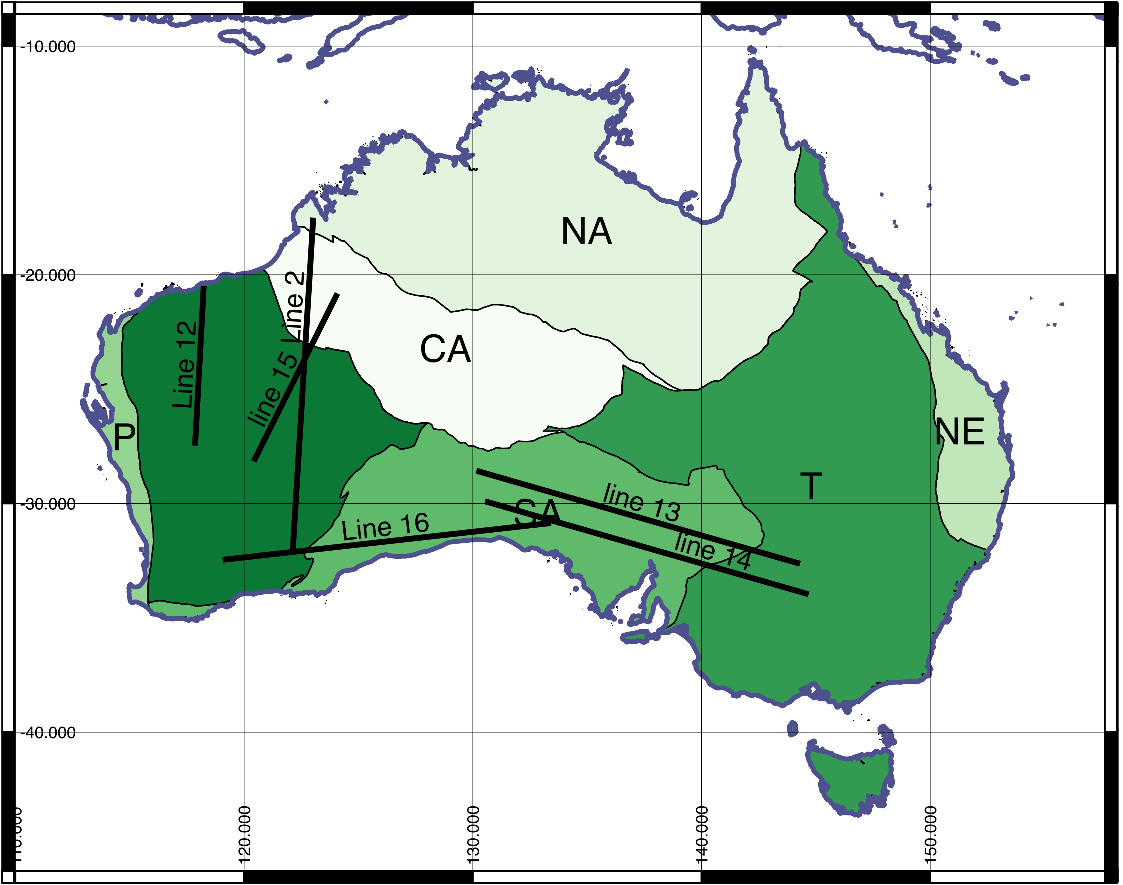
\includegraphics[width=1\linewidth]{../fig/maps/aus_lines}
	\caption[Australian lines]{Australian lines used to detect change points in this study. The polygons refers to  mayor Australian crustal elements.}
	\label{fig:aus_lines}
\end{figure}

\section{Work flow}
So far I've been using data from Geoscience Australia (Gravity 900m grid, magnetic 90m grid, and radiometric (K, Th and U, 100m grid), GOCE (gravity, 37km grid) and ADMAP (magnetic, 5km grid, in best cases). I don't have the exact reference for the data sets as they have been changing hands a few times before I got it. 

I use a GIS software (QGIS) to locate lines and sample raster vales along lines. It's fairly easy to select lines and they don't need to be straight, in case a curved line would better capture an expected boundary. The choice of lines have been discussed with Dr Jacqueline Halpin and Dr. Joanne Whittaker. When the technique is working, longer lines would be more useful.

During coding and evaluation, I've only been working on a few datasets, mainly Line 12 and 15, however, for this report I applied the method to a number of lines to guide further work: 

\begin{itemize}
	\item [2] From North to south from Kimberley into Yilgarn. 
	\item [12] Pilbara into Yilgarn.
	\item [13] Across Gawler North.
	\item [14] Across Gawler South (for reference to compare with \textit{Line 13}).
	\item [15] As 2, but perpendicular to suggested boundaries.
	\item[16] From Yilgarn, accross Albany Fraser into central South Australia. 
\end{itemize}

To shorten the processing time and to adjust resolution, the time-series are sub sampled [see figures]. Typically, when testing the code I'll sub-sample the resolution down to $1:100$, 10km, but later run typically $1:5$, 500m sampling distance. Sub-sampling is performed by applying a rolling average (essentially a LP filter) with the same window length as the sub-sampling, e.g. 5 samples. From the smoothed dataset, I pick every $n$th sample (\texttt{data[::n]}). 

The units of the data, naturally, varies in a large range and as I'm not interested in the actual data [sic] but rather the statistical changes in it. Therefore the individual datasets are normalised to a fixed range ($0-1$). 

An important watershed in change detection, is between \textit{on-line } and  \textit{off-line} methods. The first have the obvious advantage of detecting change in a stream of data, and is therefore optimized for minimal time delay. The Bayesian and Markov-chain approach works by looking at the running partition with increased scepticism but also to estimate the prior. 

I'm using a Python script to run the change-point detection. The speed depends on the square of the amount of data. That is the resolution of sample-points along lines, lengths of lines, layers of data for multivariate detection. Typically calculation time is less than one minute for a line with samples down-sampled to 1km resolution. On-line algorithm is faster than the off-line approach. Methods to speed up off-line calculations have been suggested by e.g. Xuan and Murphy \cite{Xuan2007}. There is still room for improvements in my code. 


\begin{figure}[h]
	\centering
	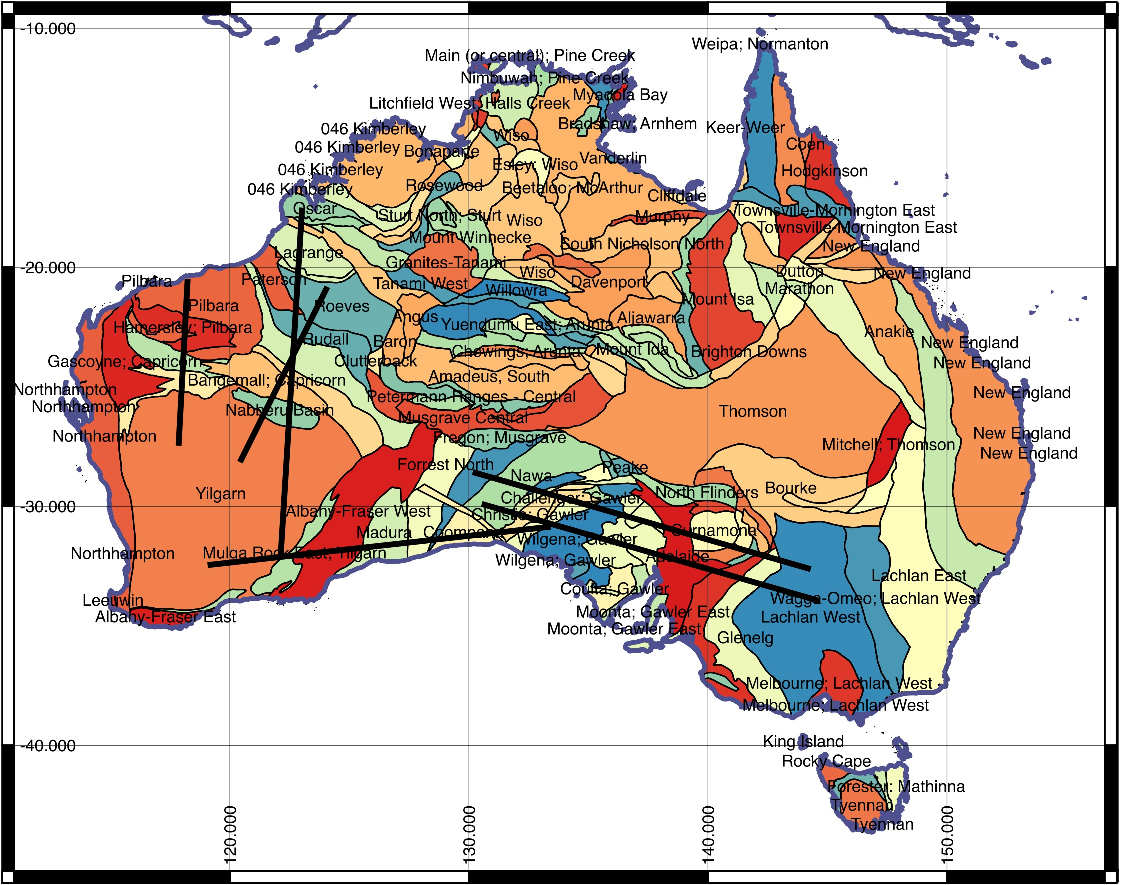
\includegraphics[width=1\linewidth]{../fig/maps/aus_geo}
	\caption[Australian geology]{The geology of Australia. The color map is trivial. These boundaries are plotted with change-points in the figures.}
	\label{fig:aus_geo}
\end{figure}



\section{Naïve techniques}
To get a first estimate of the prior function, I've been looking at the time series and calculated mean and variance over time (also known as rolling mean and roiling variance). In this example I show how average and variance of the data in 1D suggests boundaries. I also calculate the derivative of the rolling average and variance as it is the change of states I am interested in. With a number of parameters, the figures easily get clogged, but the average of the parameters gives an indication of the trends. To be useful, a weighting should be applied to the average. 

The \textit{naïve} plots are used as a reference to suggest to origin of detected change points. 

\section{On-line techniques}
I've been trying on-line techniques as they are very fast. However, there is little benefit in this application, as we know the data for the whole extension of the lines. I did not manage to create a multivariate on-line change-point detection, but that should be possible with a covariance estimate. 1-parameter off-line results are very similar to the on-line plots showed here \cite{Adams2007}. 



\section{Off-line techniques}
Off-line change-point detection would look at the whole line and use a Bayesian approach as suggested by Fearnhead \cite{Fearnhead2006} and developed by Xuan to use covariance models for multivarate data \cite{Xuan2007}. The method works well for datasets with an unknown number of change-points.
I'm using a full covariance model that have the advantage over an naïve independent features model as I expect parameters variance and mean to be linked through an unknown function rather than completely independent. Xuan and Murphy suggest a faster Gaussian graphical model that is supposed to give similar results but is much faster and might have other advantages in higher dimensions. I did not try the function yet, and it might not  be so interesting as I'll probably only use 2-4 datasets in the Antarctic application anyway. 

%\subsection{Gauss vs Xuan}





\chapter{Concerns and challenges. Room for improvements.}

Knowing that radiometric data are not available for Antarctica, I should rather rely on magnetic, gravity and possibly seismic derived data, e.g. Moho and/or LAB depth or shallow elastic properties. Subglacial topography could also be a relevant dataset, at least as a reference, maybe corrected for ice thickness. To really compare Australian with Antarctic data, I will use global datasets to mitigate the effects of different resolution. However, at this point I still find it useful to refer to the high resolution Australian data. 

Change point detection is by it's nature a 1D method, traditionally used for time series. I, so far, use extracted time series from 2D datasets. However, I'm worried that artefacts form acquisition and processing have a large impact. E.g. missing data will directly be interpreted as a change-point in most cases and changes in acquisition methods, e.g. between high resolution airborne magnetic data vs. low resolution satellite data in the ADMAP dataset. In the case of Antarctica, this can be improved by use of new high resolution datasets for gravity and magnetism. 

Finally, smoothing and other filtering of the original 2D datasets are common, but can also affect the detected change-points. Only necessary processing should be applied to the datasets used. Some noise depends on geological factors.

The processed data is (from Reading and Gallagher (2013) \cite{Reading2013}): 

\begin{equation}
\sigma^2_{T} =\sigma^2_{GP} + \sigma^2_{GN}  + \sigma^2_{AN}
\end{equation}

$\sigma^2_{GP} $ and $\sigma^2_{GN} $ represent the actual earth, but the analytical and technical noise, $\sigma^2_{AN}$, would be a more important factor in the spatial application. 

In this unscaled application. $GP$ could be imagined representing geological terrain boundaries and $GN$ the local geology, sedimentary cover and anomalies. 

$\sigma^2_{AN}$  \textit{contains}:
\begin{enumerate}
	
	\item Geometric limitation in datasets, spatial frequency distribution.
	\item Information derived from instrumentation. 
	\item Data gaps. Could be solved by implementing Xie's (2013) \cite{Xie2013}
	\item Information derived from interpolation, when 1D datasets were compiled to 2D.
	\item Information derived from corrections, eg. Bouguer correction. 

\end{enumerate}

Weighting and normalisation of datasets is also an issue that should ve discussed and tested. I'm using a basic peak-to-peak algorithm, (\texttt{(x - x.min()) / (x.max() - x.min())}) but I guess that an actual scaling parameter based on the content of the data would be better. 




\chapter{To do.}

The todo list

\begin{enumerate}
	\item Apply methods on consistent, global, datasets over Antarctica and Australia. At the moment accept the lower resolution, but as next step try to apply the developed methods on high resolution data (e.g. ICECAP and ADMAP2)
	
	\item Look at methods to weight the datasets. E.g. use different conditional priors for different data. 
	
	\item Compare 1D changepoint detection with 2D methods, e.g. worming (e.g. \cite{Australia2013, fitzgerald2006innovative}). Basic slope maps and second order slope maps, change of change rate. By higher derivation of data, it could be possible to map the changes in the 2D plane. 
	
	\item Improve prior function. Instead of the constant prior, used in this report, a geometric prior based on geological expectation should be tested. 
	
	\item Speed up the computations by compile central functions. 
	
	\item Investigate weighting of data and normalization. 
	
	\item A few recent studies have introduced additional improvements that I'm trying to implement. \cite{Matteson1306} uses hierarchical clustering to find multivariate changepoints in an off-line approach with rather promising results.  \cite{Xie2013} suggests methods to deal with data gaps and missing elements in higher dimension. This might suggest ways to develop a fully analytic 2D approach without interpolation, if based on 2D datasets. \cite{Harle2014} combines robust local statistic analysis with an Bayesian overview. This might be a good method for spatial data as I often get false-hits in the vicinity of the actual change. 
\end{enumerate}





%The delineations between partitions are called the changepoints.We further assume that for each partition ρ, the data within it are i.i.d. from some probability distribution P (xt | ηρ). The parameters ηρ, ρ = 1, 2, . . . are taken to be i.i.d. as well. We denote the contiguous set of observations between time a and b inclusive as xa:b. The discrete a priori probability distribution over the interval between changepoints is denoted as Pgap(g).







%Offline Changepoint Detection
%Lets compute the probability of changepoints at each time step. We need two things for that. First a prior of how probable is it to have two successive changepoints with the distance t. The second thing is a model of the likelihood of data in a sequence [s, t] of the data, given that in this sequence there is no changepoint.
%For this example we assume a uniform prior over the length of sequences (const_prior) and a piecewise gaussian model (gaussian_obs_log_likelihood).


%Use SSE accelerated logsumexp().
%The offline_changepoint_detection() function returns three things: Q[t], the log-likelihood of data [t, n], P[t, s], the log-likelihood of a datasequence [t, s], given there is no changepoint between t and s and Pcp[i, t], the log-likelihood that the i-th changepoint is at time step t. To actually get the probility of a changepoint at time step t sum the probabilities.

%That works pretty well, but is somewhat slow. It's possible to speed that up by truncating a sum in the algorithm. However that sometimes leeds to $\infty$ values. Set the truncate parameter to e.g. -10 to test that out.

%[1] Paul Fearnhead, Exact and Efficient Bayesian Inference for Multiple Changepoint problems, Statistics and computing 16.2 (2006), pp. 203--213
%[2] Xuan Xiang, Kevin Murphy, Modeling Changing Dependency Structure in Multivariate Time Series, ICML (2007), pp. 1055--1062

%Online Changepoint Detection
%Let's assume the data points come in one after another and not as these nice batches. During the process you want to know if the new point has the same hyperparameter or different ones. You need an online changepoint detection.
%Happily there is one, although it's interface is kind of suboptimal so far, in that it expects batches of data still and just assumes they drop in over time... I will change that at some point.
%The online version computes slightly different things. For each time step it returns the probability distribution over the length of the last sequence. E.g. R[7, 3] is the probability at time step 7 that the last sequence is already 3 time steps long. It also returns the MAP estimate at each timestep for convenience.
%To plot the distributions we use a grey-scale colormap, black is zero, white 1. We also plot the probability at each time step for a sequence length of 0, i.e. the probability of the current time step to be a changepoint.
%Because it's very hard to correctly evaluate a change after a single sample of a new distribution, we instead can "wait" for Nw samples and evalute the probability of a change happening Nw samples prior.

%[1] Ryan P. Adams, David J.C. MacKay, Bayesian Online Changepoint Detection, arXiv 0710.3742 (2007)
%There you also find a Matlab version, which this code is based on.

%[1] Paul Fearnhead, Exact and Efficient Bayesian Inference for Multiple
%Changepoint problems, Statistics and computing 16.2 (2006), pp. 203--213

%[2] Ryan P. Adams, David J.C. MacKay, Bayesian Online Changepoint Detection,
%arXiv 0710.3742 (2007)

%[3] Xuan Xiang, Kevin Murphy, Modeling Changing Dependency Structure in
%Multivariate Time Series, ICML (2007), pp. 1055--1062





\chapter{Temporary results}
The lines are analysed as 550m sampling distance. (1:5 sub-sampling) and 5.5km (1:50 sub-sampling) sampling distance. The re-sampling is combined with a low-pass filter through rolling average and suggest the accuracy of the method for global low-resolution data. 

For the on-line detection a wait time of 80 samples was used \cite{Adams2007}. The Off-line detection used constant prior and full covariance model. Truncation at -100. \cite{Xuan2011,Xuan2007,Fearnhead2006}. \\

The run time for all results in this report, was 672s  in a parallel build on 6 cores. 2.6 GHz Intel Core i7, 16Gb. 

Maps are generated in QGIS, but colour maps is trivial and names refers to Geo-science Australia terrain map, as also used as references in the figures. 

\begingroup
\let\clearpage\relax
\listoffigures
\endgroup

\begin{figure}[h]
	\centering
	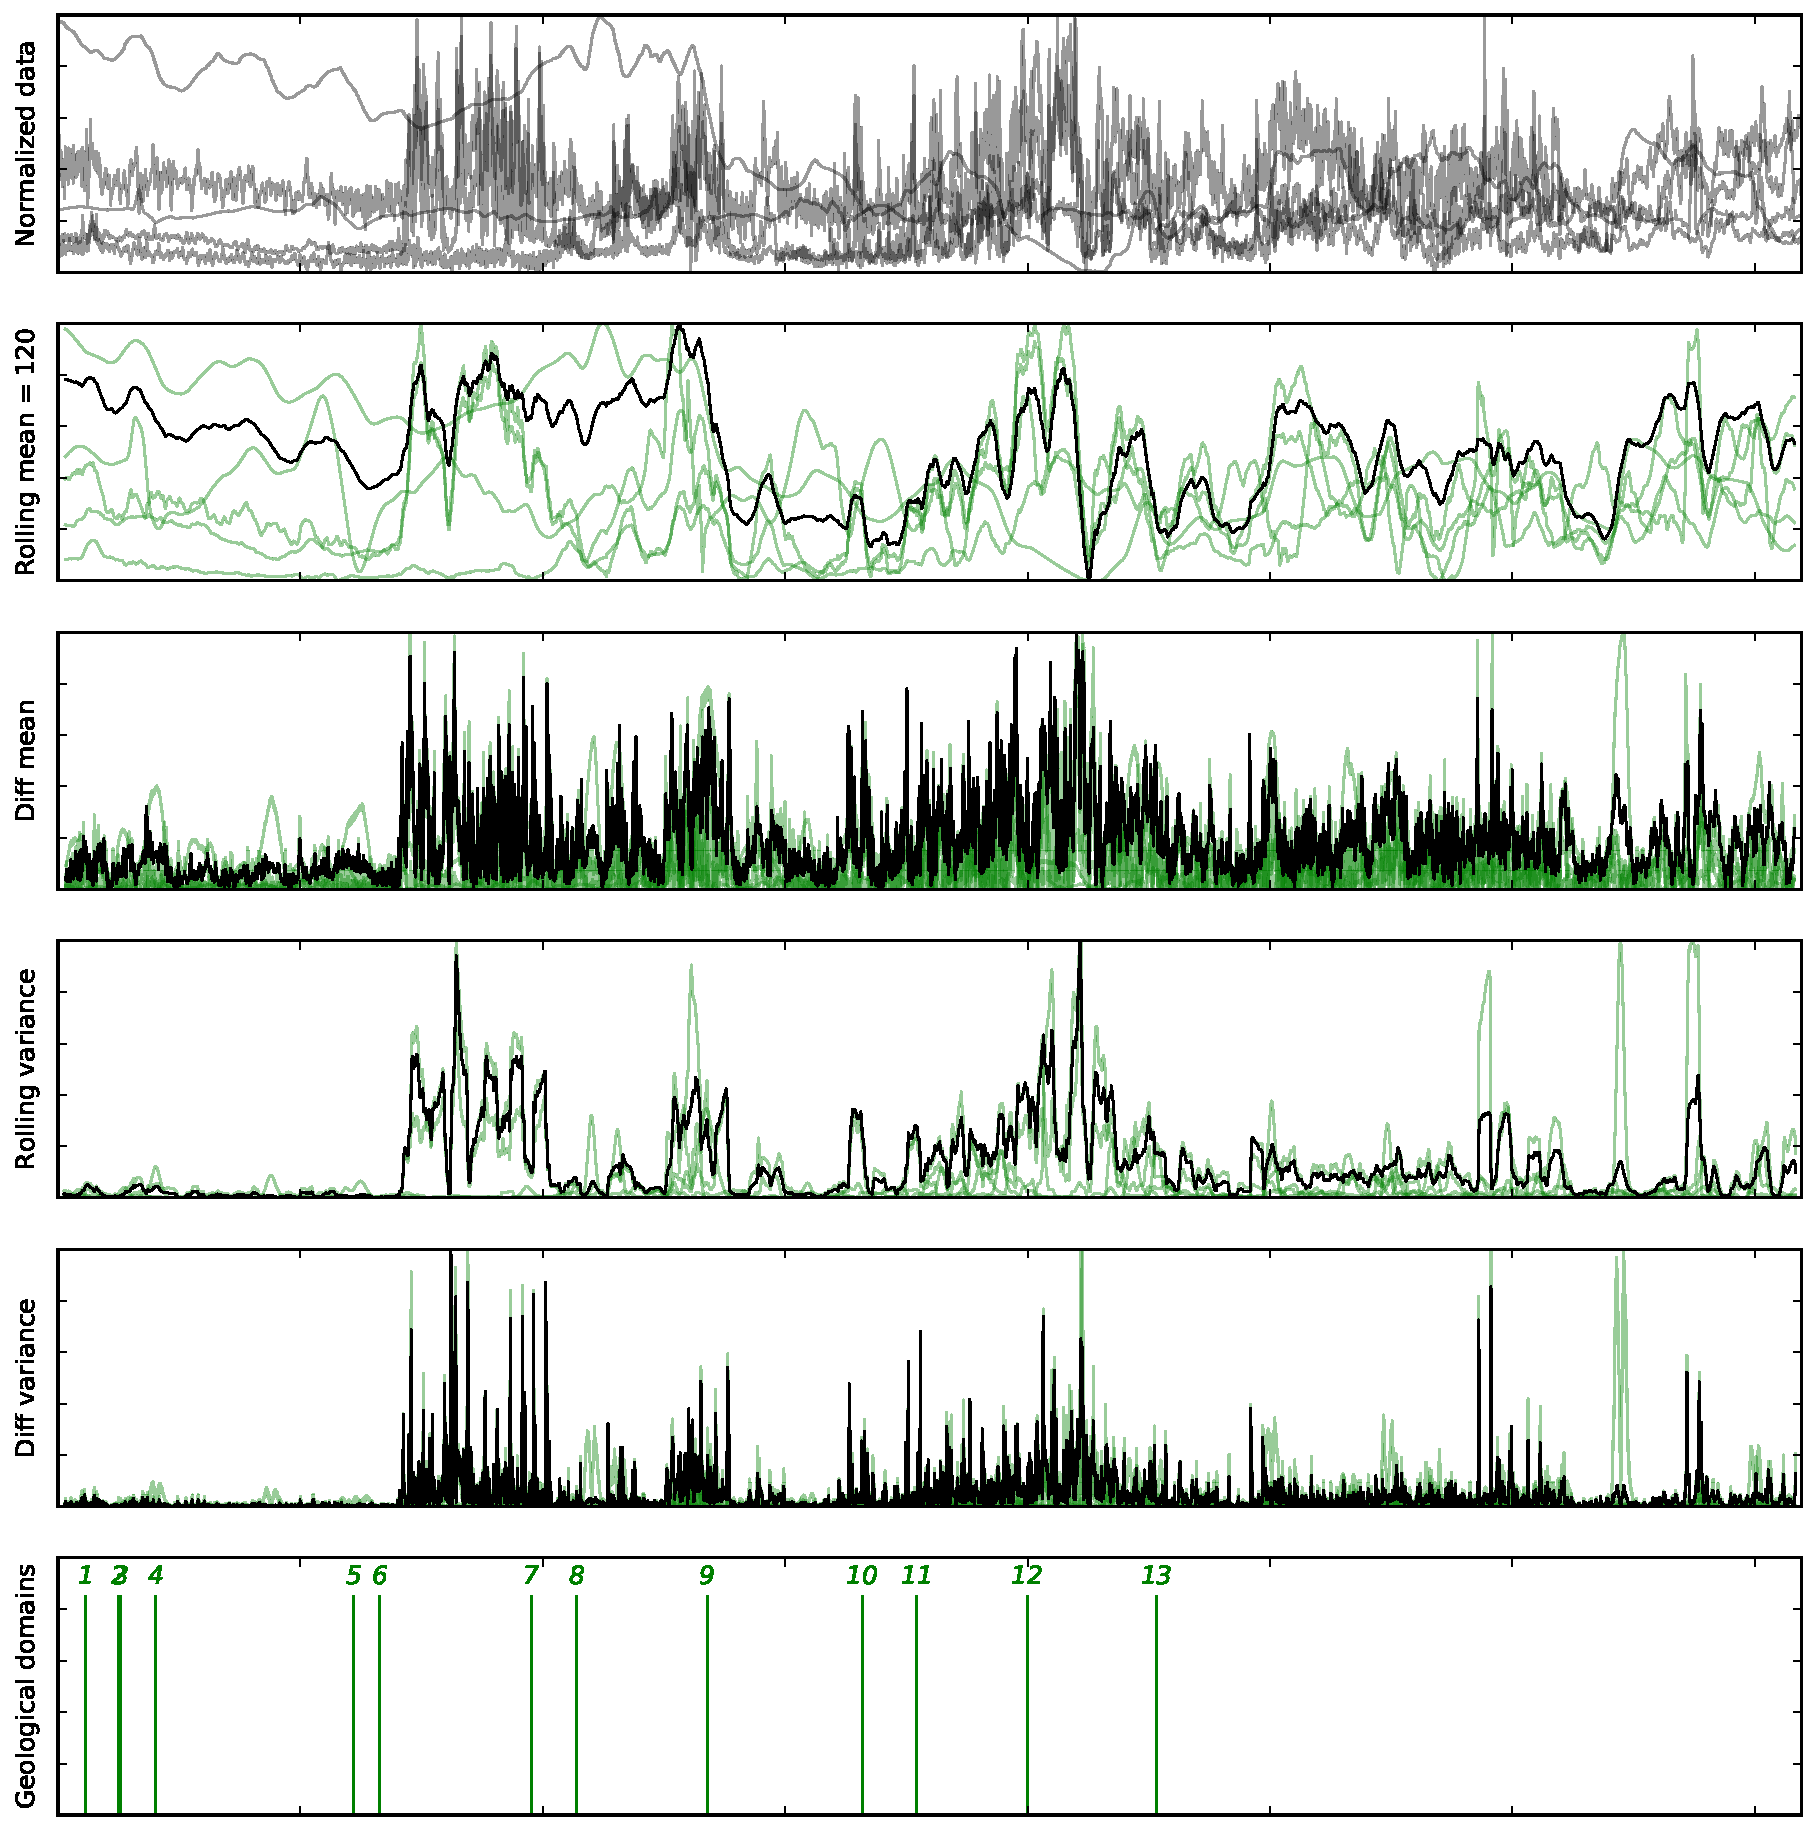
\includegraphics[width=1\linewidth]{../fig/naive_ga_vpt_line_2}
	\caption[Naïve 2]{Statistic analysis of Line 2. From left: Oscar Range region, basement province, 1: Nookanbah (250k) region, basement province, 2: Basement to Barbwire Terrace of 017 Canning Basin, 3: Lagrange (250k map) region, basement province, 4: Koop 100k map region (geophysicallly overprinted zone); basement province, 5: Roeves (gravity feature, Reeves Knoll) region; basement province, 6: 067 Paterson Province, 7: Rudall Inlier within  067 Paterson Province, 8: LD Lake Dissapointment  region (Gunanya 1:250k map); 067 Paterson Province (?), 9: Capricorn East (geophysical) region of Capricorn Orogen (e.g., Trainor 100k map); basement province (poorly defined), 10: Basement to 011 Bangemall Basin; Capricorn Orogen, 11: Overlies NE Yilgarn, 12: 093 Yilgarn Craton (Super)-province (Block)
}
	\label{fig:naive2}
\end{figure}


\begin{figure}[h]
	\centering
	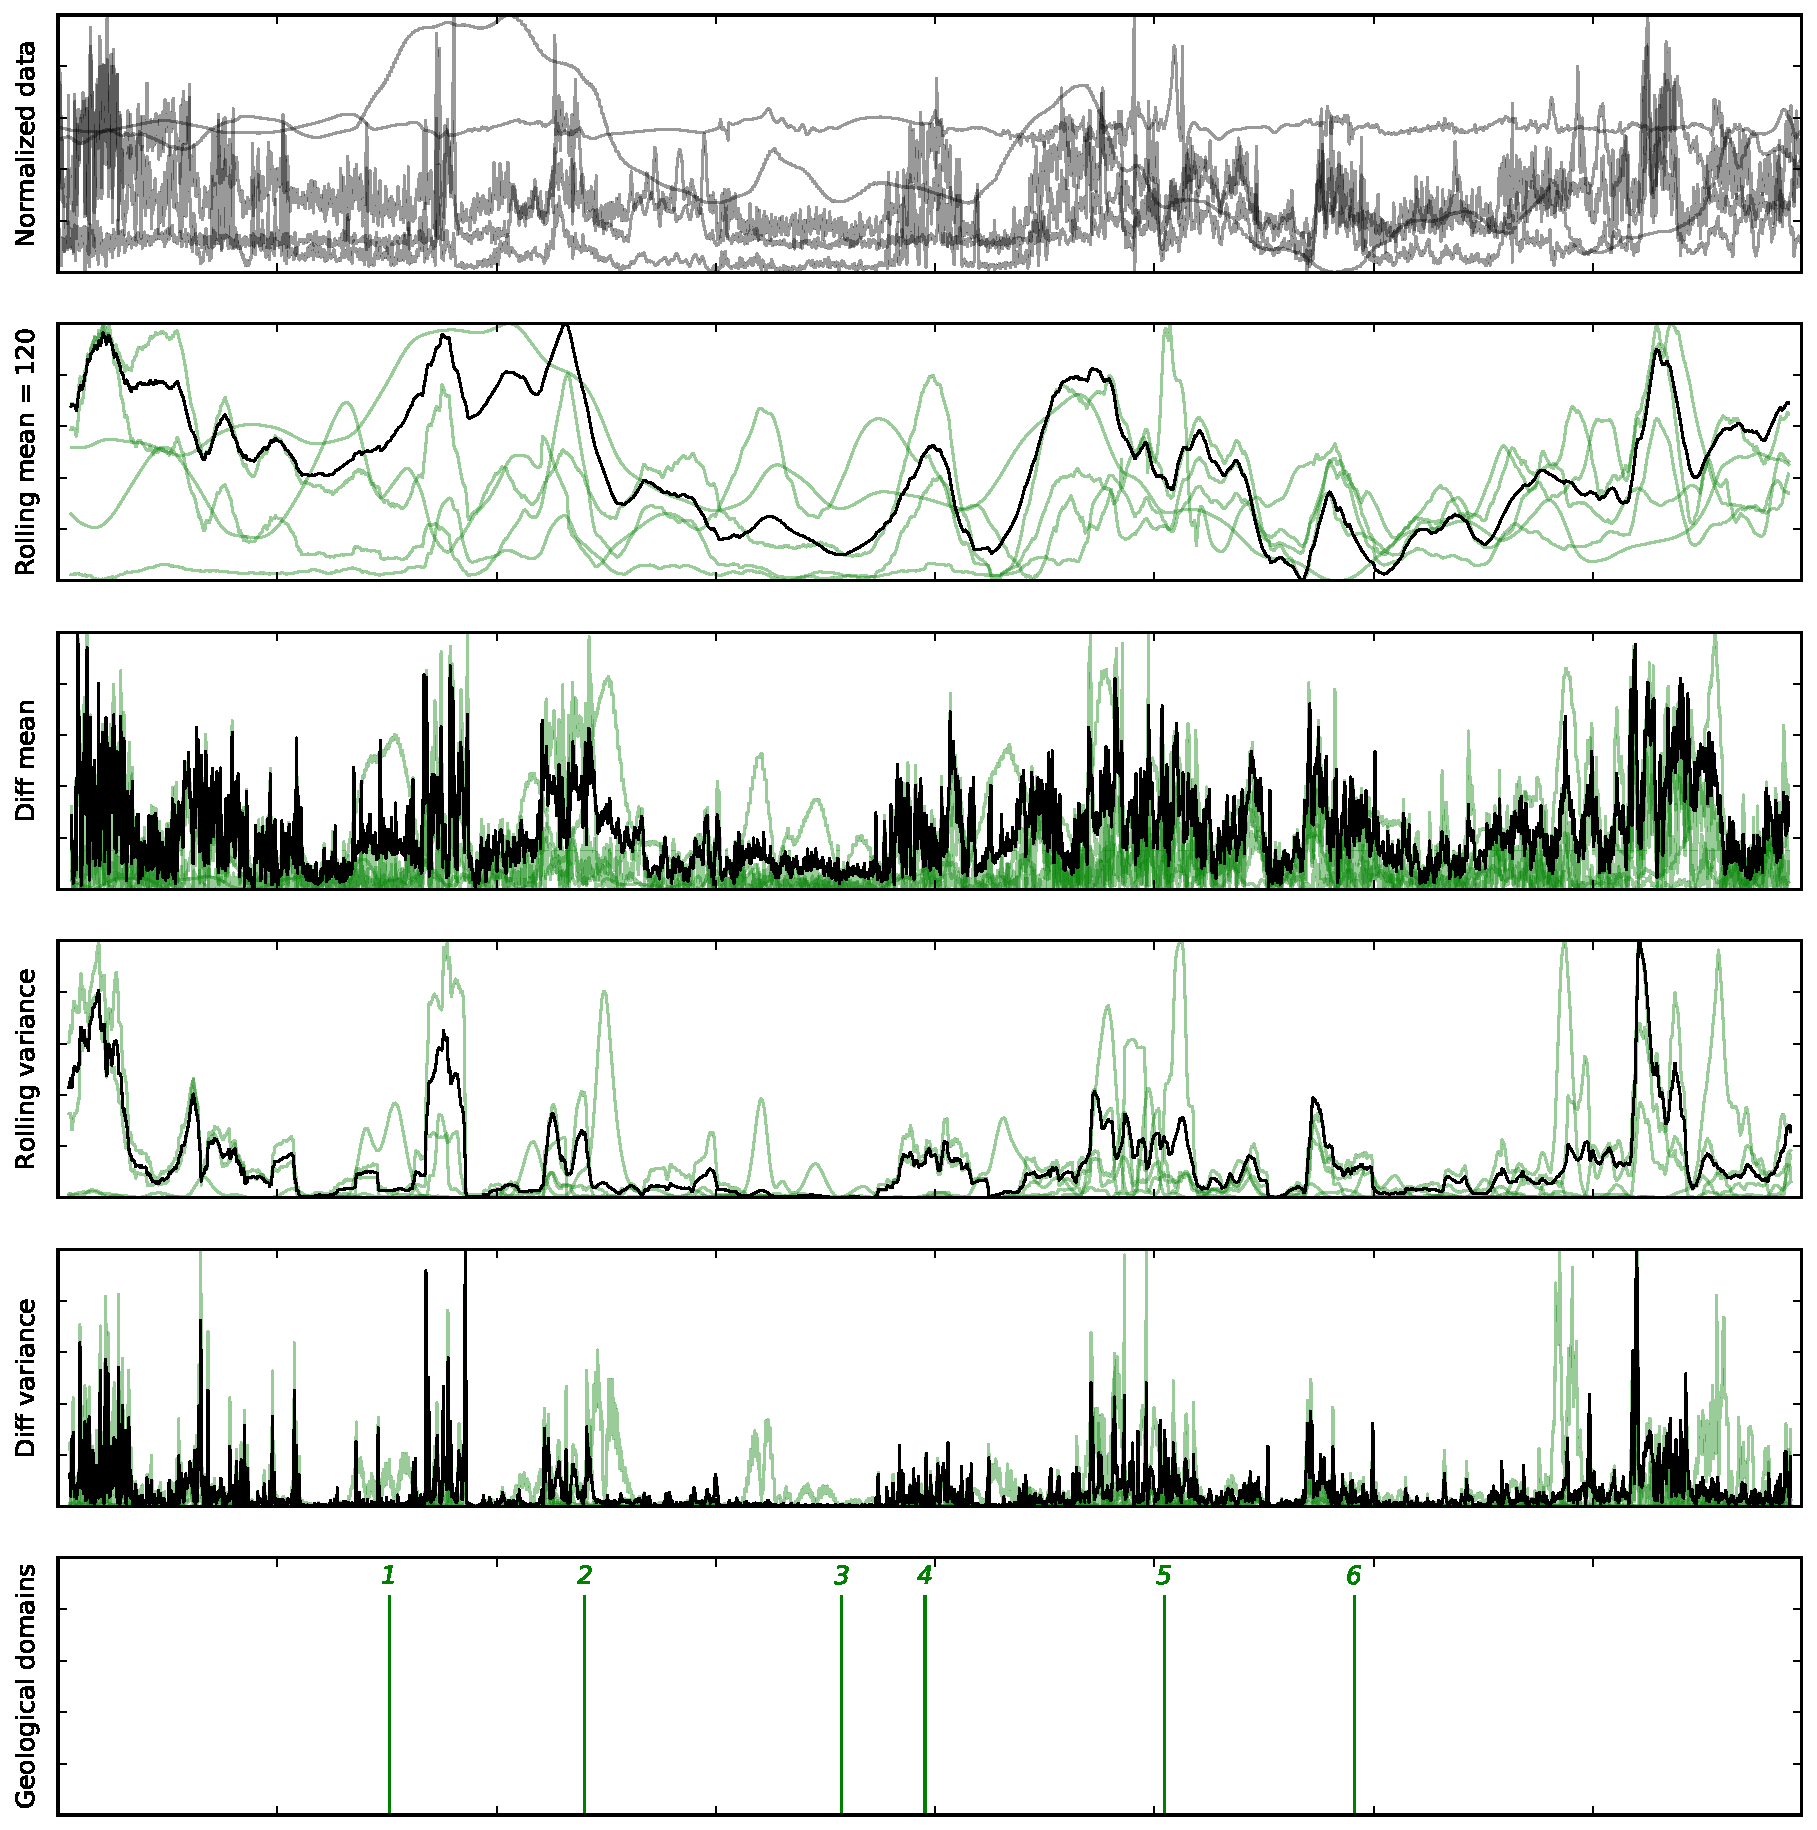
\includegraphics[width=1\linewidth]{../fig/naive_ga_vpt_line_15}
	\caption[Naïve 15]{Statistic analysis of Line 15. From left: Roeves (gravity feature, Reeves Knoll) region; basement province, 1: Rudall Inlier within  067 Paterson Province, 2: LD Lake Dissapointment  region (Gunanya 1:250k map); 067 Paterson Province (?), 3: Capricorn East (geophysical) region of Capricorn Orogen (e.g., Trainor 100k map); basement province (poorly defined), 4: Basement to 011 Bangemall Basin; Capricorn Orogen, 5: Overlies NE Yilgarn, 6: 093 Yilgarn Craton (Super)-province (Block)
}
	\label{fig:naive15}
\end{figure}

\begin{figure}[h]
	\centering
	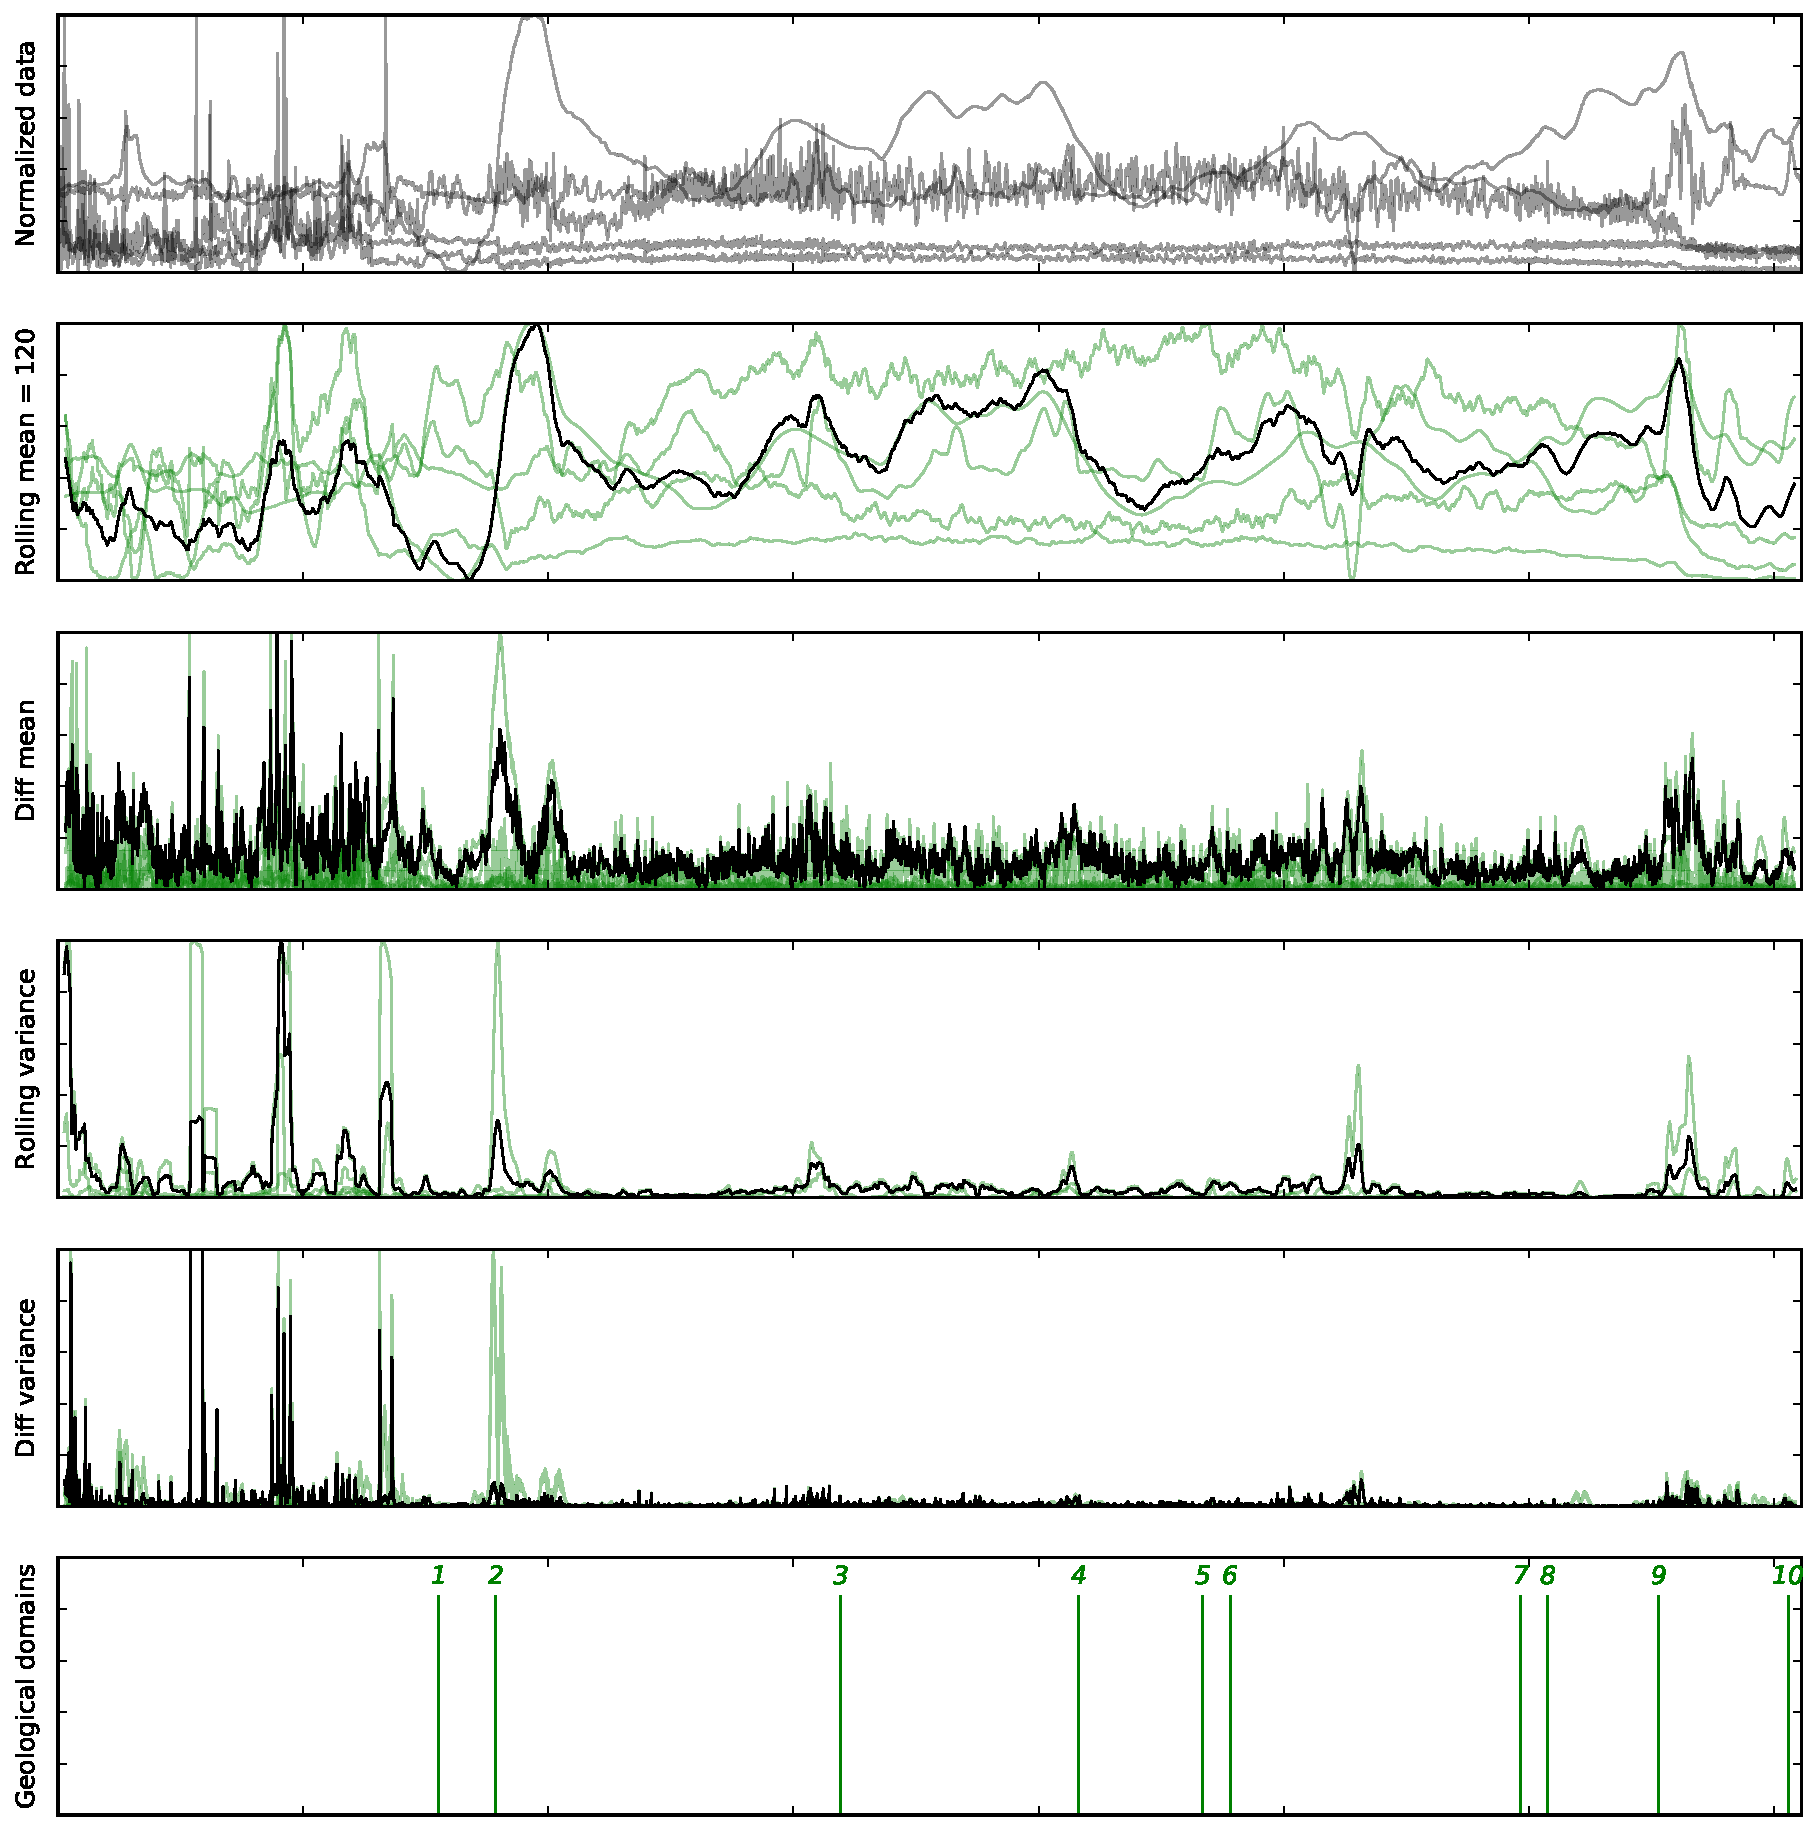
\includegraphics[width=1\linewidth]{../fig/naive_ga_vpt_line_16}
	\caption[Naïve 16]{Statistic analysis of Line 16. From left: 093 Yilgarn Craton (Super)-province (Block), 1: Mulga Rock (overprinted geophysical) zone; 093 Yilgarn (Super) province, 2: 003 Albany-Fraser Province, 3: Madura (250k map) region (or Naretha region); basement province, 4: Forrest (250k map) region, basement province, 5: Waigen (250k map) region; basement province, 6: Coompana Province (Block); basement province, 7: Cook (geophysically overprinted) zone (e.g., Cook 100k map); dolerite dyke swarm at northern edge of Coompana Block, basement unit (WT: Watson zone in version-1 map), 8: Christie structural subdomain (Barton 250k map); 036 Gawler Craton, 9: Fowler zone (Colona and Coorambie Fault zones), eastern Christie structural subdomain (NW Fowler 250k map); 036 Gawler Craton, 10: Wilgena and Nuyts structural subdomains; 036 Gawler Craton
}
	\label{fig:naive16}
\end{figure}

\begin{figure}[h]
\centering
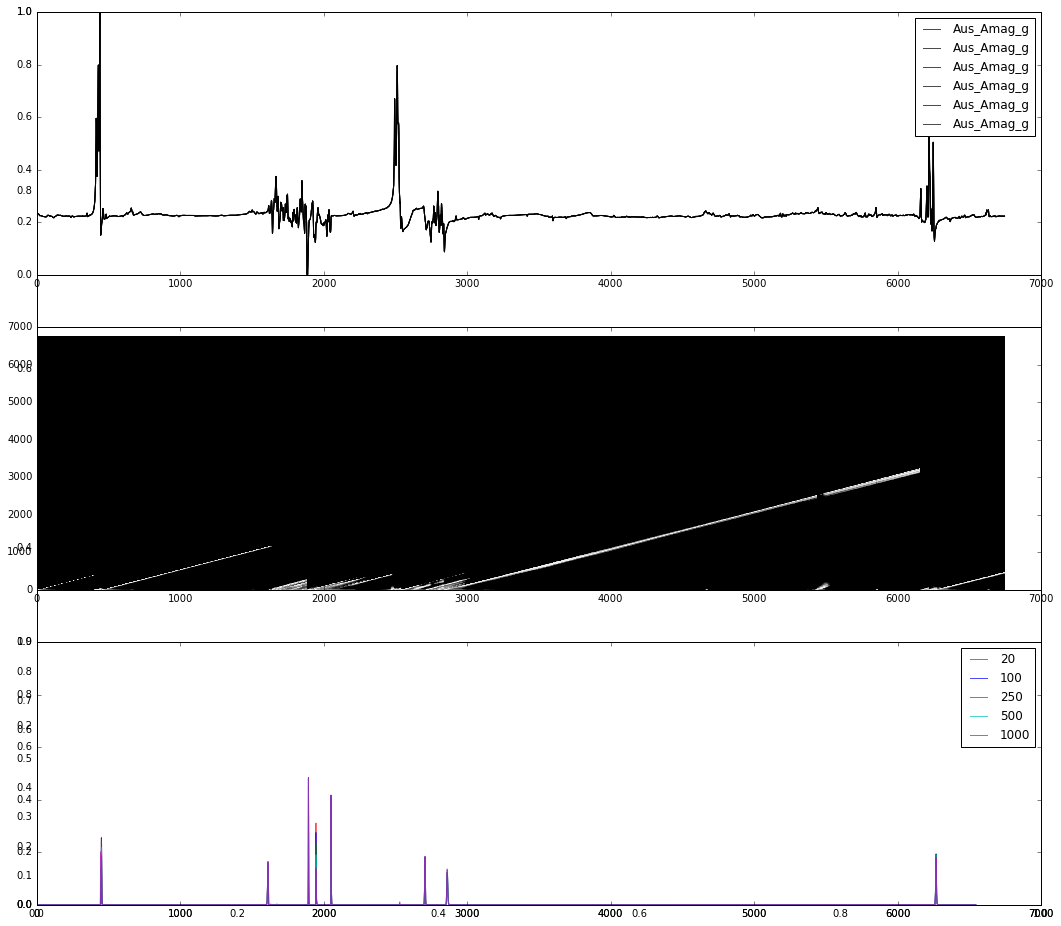
\includegraphics[width=1\linewidth]{../fig/1v_12_hi_Nw}
\caption[On-line changepoint detection. Line 12 (1:5)]{Online changepoint detection for Line 12. Upper plot shows all potential field data. Mid plot schow posterior probability based on magnetic data. A new run starts at each changepoint. Lower plot shows changepoint probability based on only magnetic data.}
\label{fig:1v12hinw}
\end{figure}

\begin{figure}
	\centering
	\begin{subfigure}[b]{1\textwidth}
		\centering
		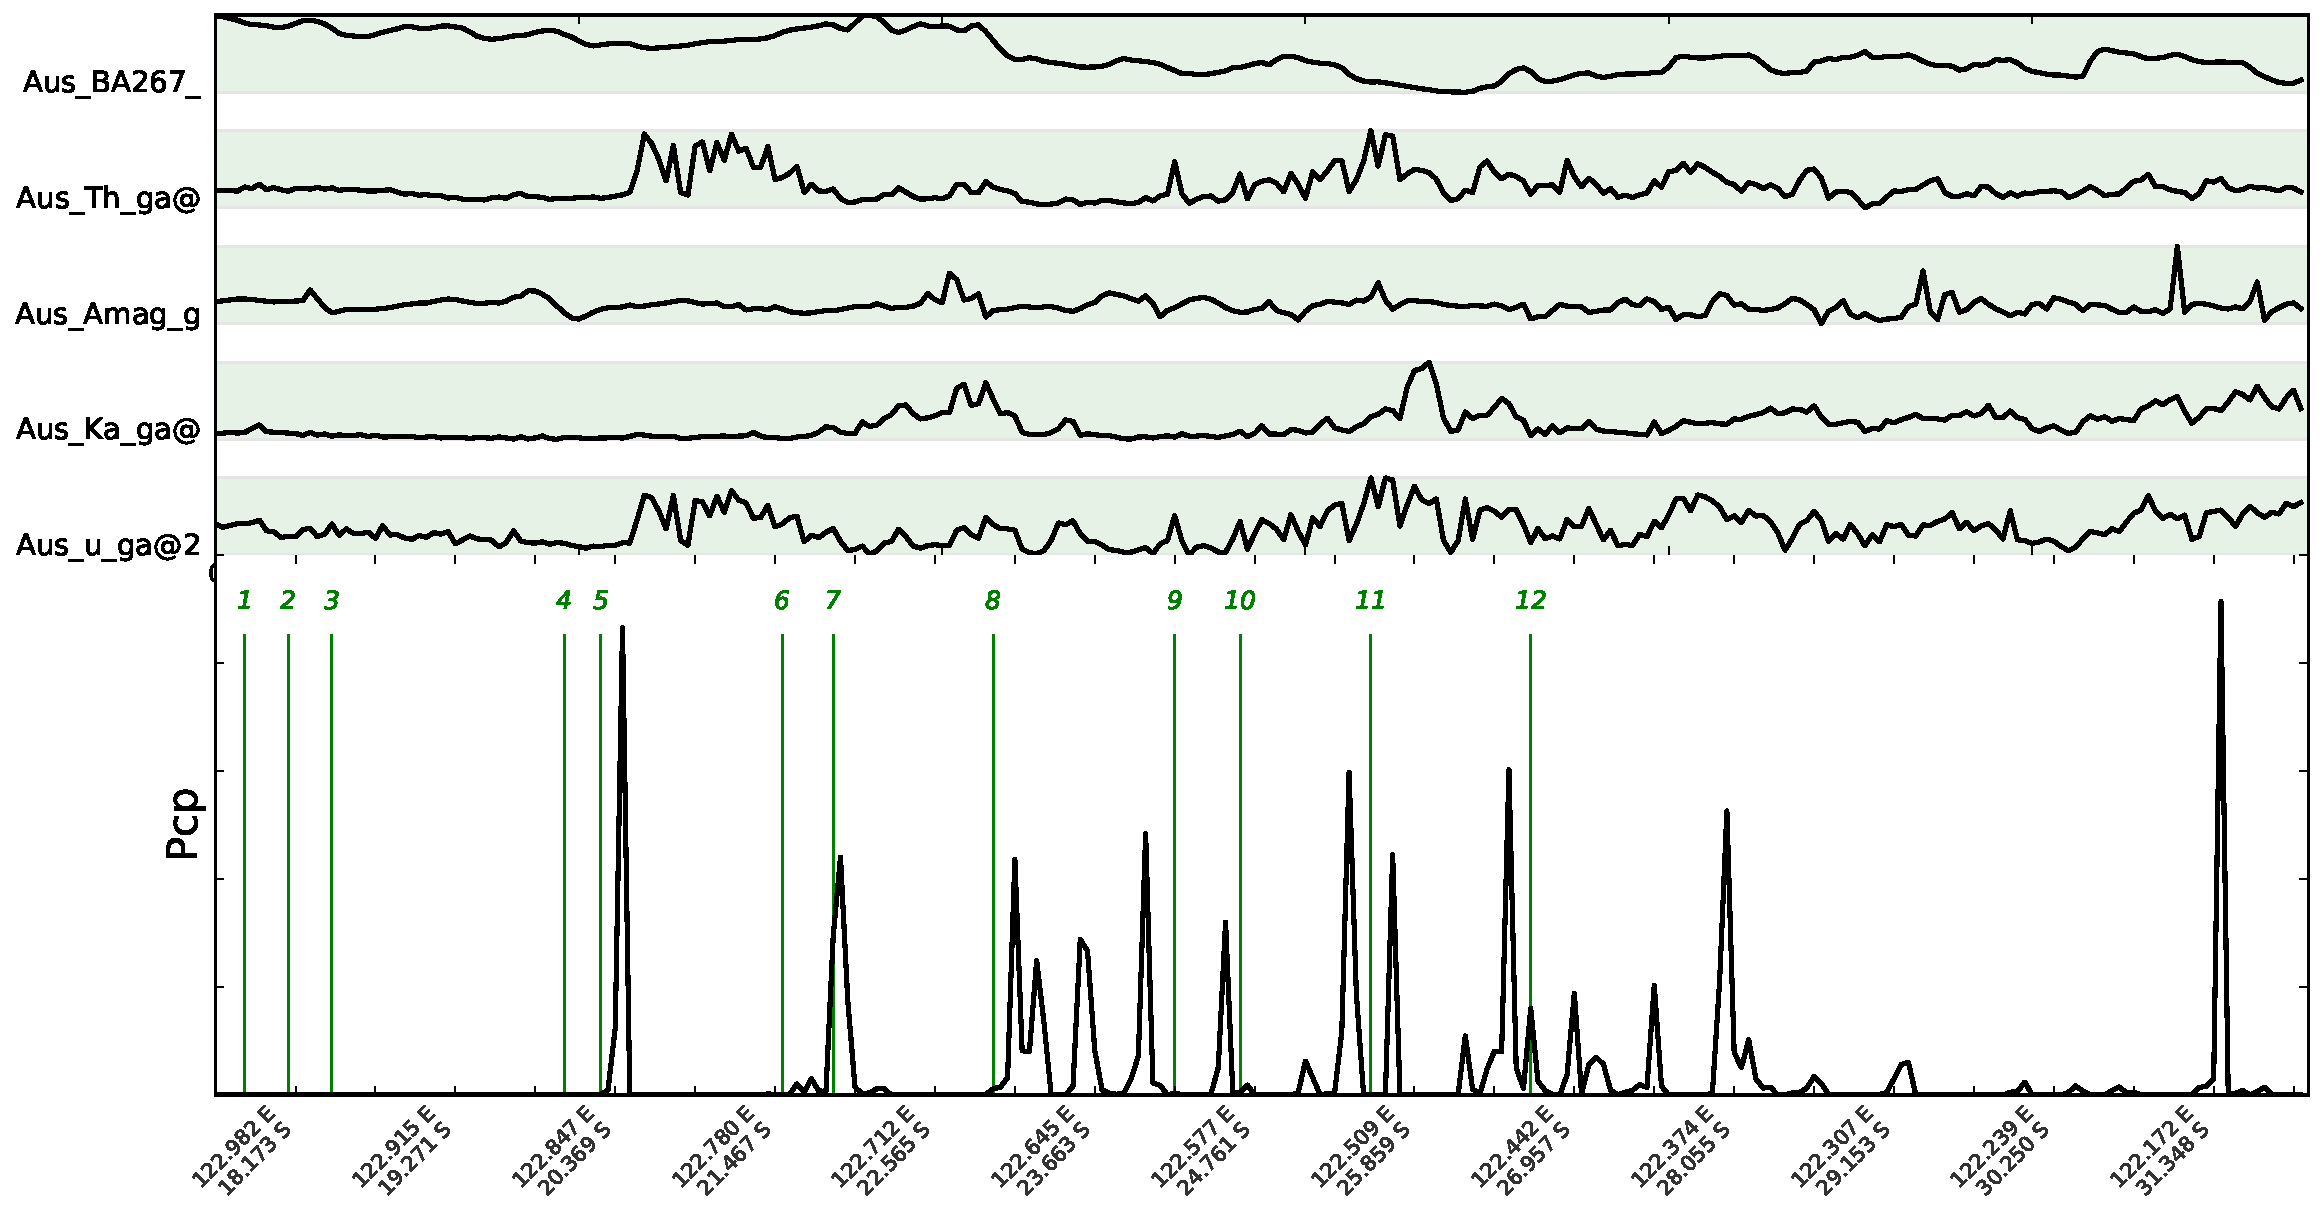
\includegraphics[width=0.9\linewidth]{../fig/ga_vpt_line_2}
		\caption[Line 2]{Line 2 subsampled 1:5 From left: Oscar Range region, basement province, 1: Nookanbah (250k) region, basement province, 2: Basement to Barbwire Terrace of 017 Canning Basin, 3: Lagrange (250k map) region, basement province, 4: Koop 100k map region (geophysicallly overprinted zone); basement province, 5: Roeves (gravity feature, Reeves Knoll) region; basement province, 6: 067 Paterson Province, 7: Rudall Inlier within  067 Paterson Province, 8: LD Lake Dissapointment  region (Gunanya 1:250k map); 067 Paterson Province (?), 9: Capricorn East (geophysical) region of Capricorn Orogen (e.g., Trainor 100k map); basement province (poorly defined), 10: Basement to 011 Bangemall Basin; Capricorn Orogen, 11: Overlies NE Yilgarn, 12: 093 Yilgarn Craton (Super)-province (Block)
}
		\label{fig:galine2}
	\end{subfigure}
	
	\begin{subfigure}[b]{1\textwidth}
		\centering
		\includegraphics[width=0.9\linewidth]{../fig/ga_vpt_line_2_lo}
		\caption[Line 2]{Line 2 subsampled 1:50 From left: Oscar Range region, basement province, 1: Nookanbah (250k) region, basement province, 2: Basement to Barbwire Terrace of 017 Canning Basin, 3: Lagrange (250k map) region, basement province, 4: Koop 100k map region (geophysicallly overprinted zone); basement province, 5: Roeves (gravity feature, Reeves Knoll) region; basement province, 6: 067 Paterson Province, 7: Rudall Inlier within  067 Paterson Province, 8: LD Lake Dissapointment  region (Gunanya 1:250k map); 067 Paterson Province (?), 9: Capricorn East (geophysical) region of Capricorn Orogen (e.g., Trainor 100k map); basement province (poorly defined), 10: Basement to 011 Bangemall Basin; Capricorn Orogen, 11: Overlies NE Yilgarn, 12: 093 Yilgarn Craton (Super)-province (Block)
}
		\label{fig:galine2_lo}
	\end{subfigure}
	
	\caption[Line 2]{Line 2}
\end{figure}

\begin{figure}
	\centering
	\begin{subfigure}[b]{1\textwidth}
		\centering
		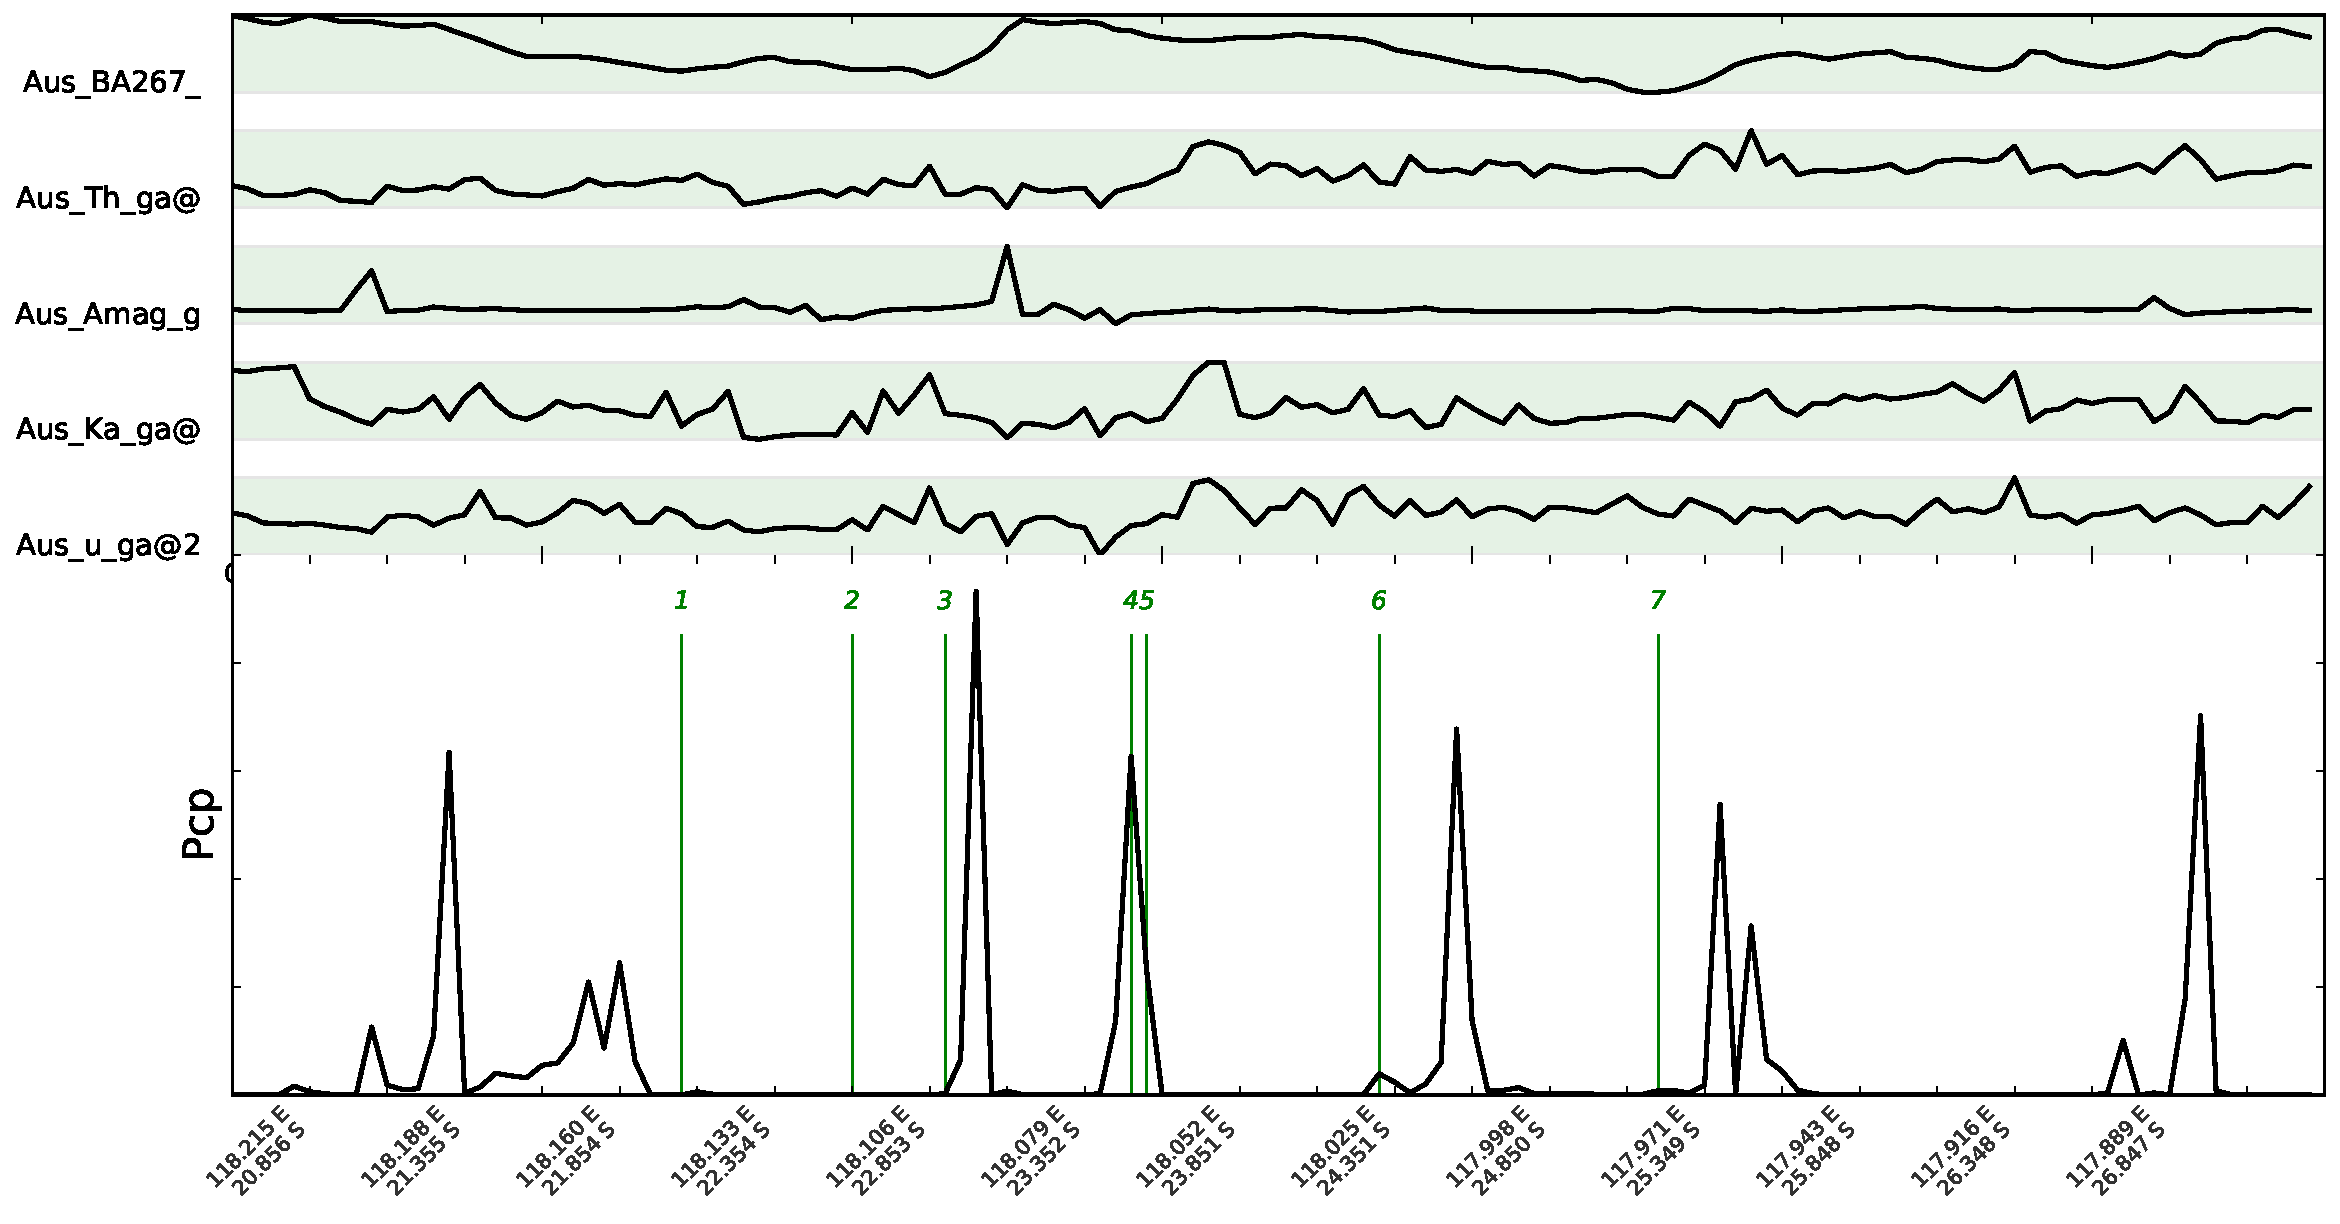
\includegraphics[width=0.9\linewidth]{../fig/ga_vpt_line_12}
		\caption[Line 12]{Line 12 subsampled 1:5 From left: 070 Pilbara Province (Craton/ Block), 1: 041 Hamersley Basin; overlies 070 Pilbara Craton, 2: 070 Pilbara Province (Craton/ Block), 3: 041 Hamersley Basin; overlies 070 Pilbara Craton, 4: 070 Pilbara Province (Craton/ Block), 5: Mount Vernon (100k map) region; 112 Asburton Basin; marginal to Capricorn Orogen, 6: Collier (250k map) region of Capricorn Orogen; southern 035 Gascoyne Province, 7: 093 Yilgarn Craton (Super)-province (Block)
}
		\label{fig:galine12}
	\end{subfigure}
	
	\begin{subfigure}[b]{1\textwidth}
		\centering
		\includegraphics[width=0.9\linewidth]{../fig/ga_vpt_line_12_lo}
		\caption[Line 12]{Line 12 subsampled 1:50 From left: 070 Pilbara Province (Craton/ Block), 1: 041 Hamersley Basin; overlies 070 Pilbara Craton, 2: 070 Pilbara Province (Craton/ Block), 3: 041 Hamersley Basin; overlies 070 Pilbara Craton, 4: 070 Pilbara Province (Craton/ Block), 5: Mount Vernon (100k map) region; 112 Asburton Basin; marginal to Capricorn Orogen, 6: Collier (250k map) region of Capricorn Orogen; southern 035 Gascoyne Province, 7: 093 Yilgarn Craton (Super)-province (Block)
}
		\label{fig:galine12_lo}
	\end{subfigure}
	
	\caption[Line 12]{Line 12}
\end{figure}

\begin{figure}
	\centering
	\begin{subfigure}[b]{1\textwidth}
		\centering
		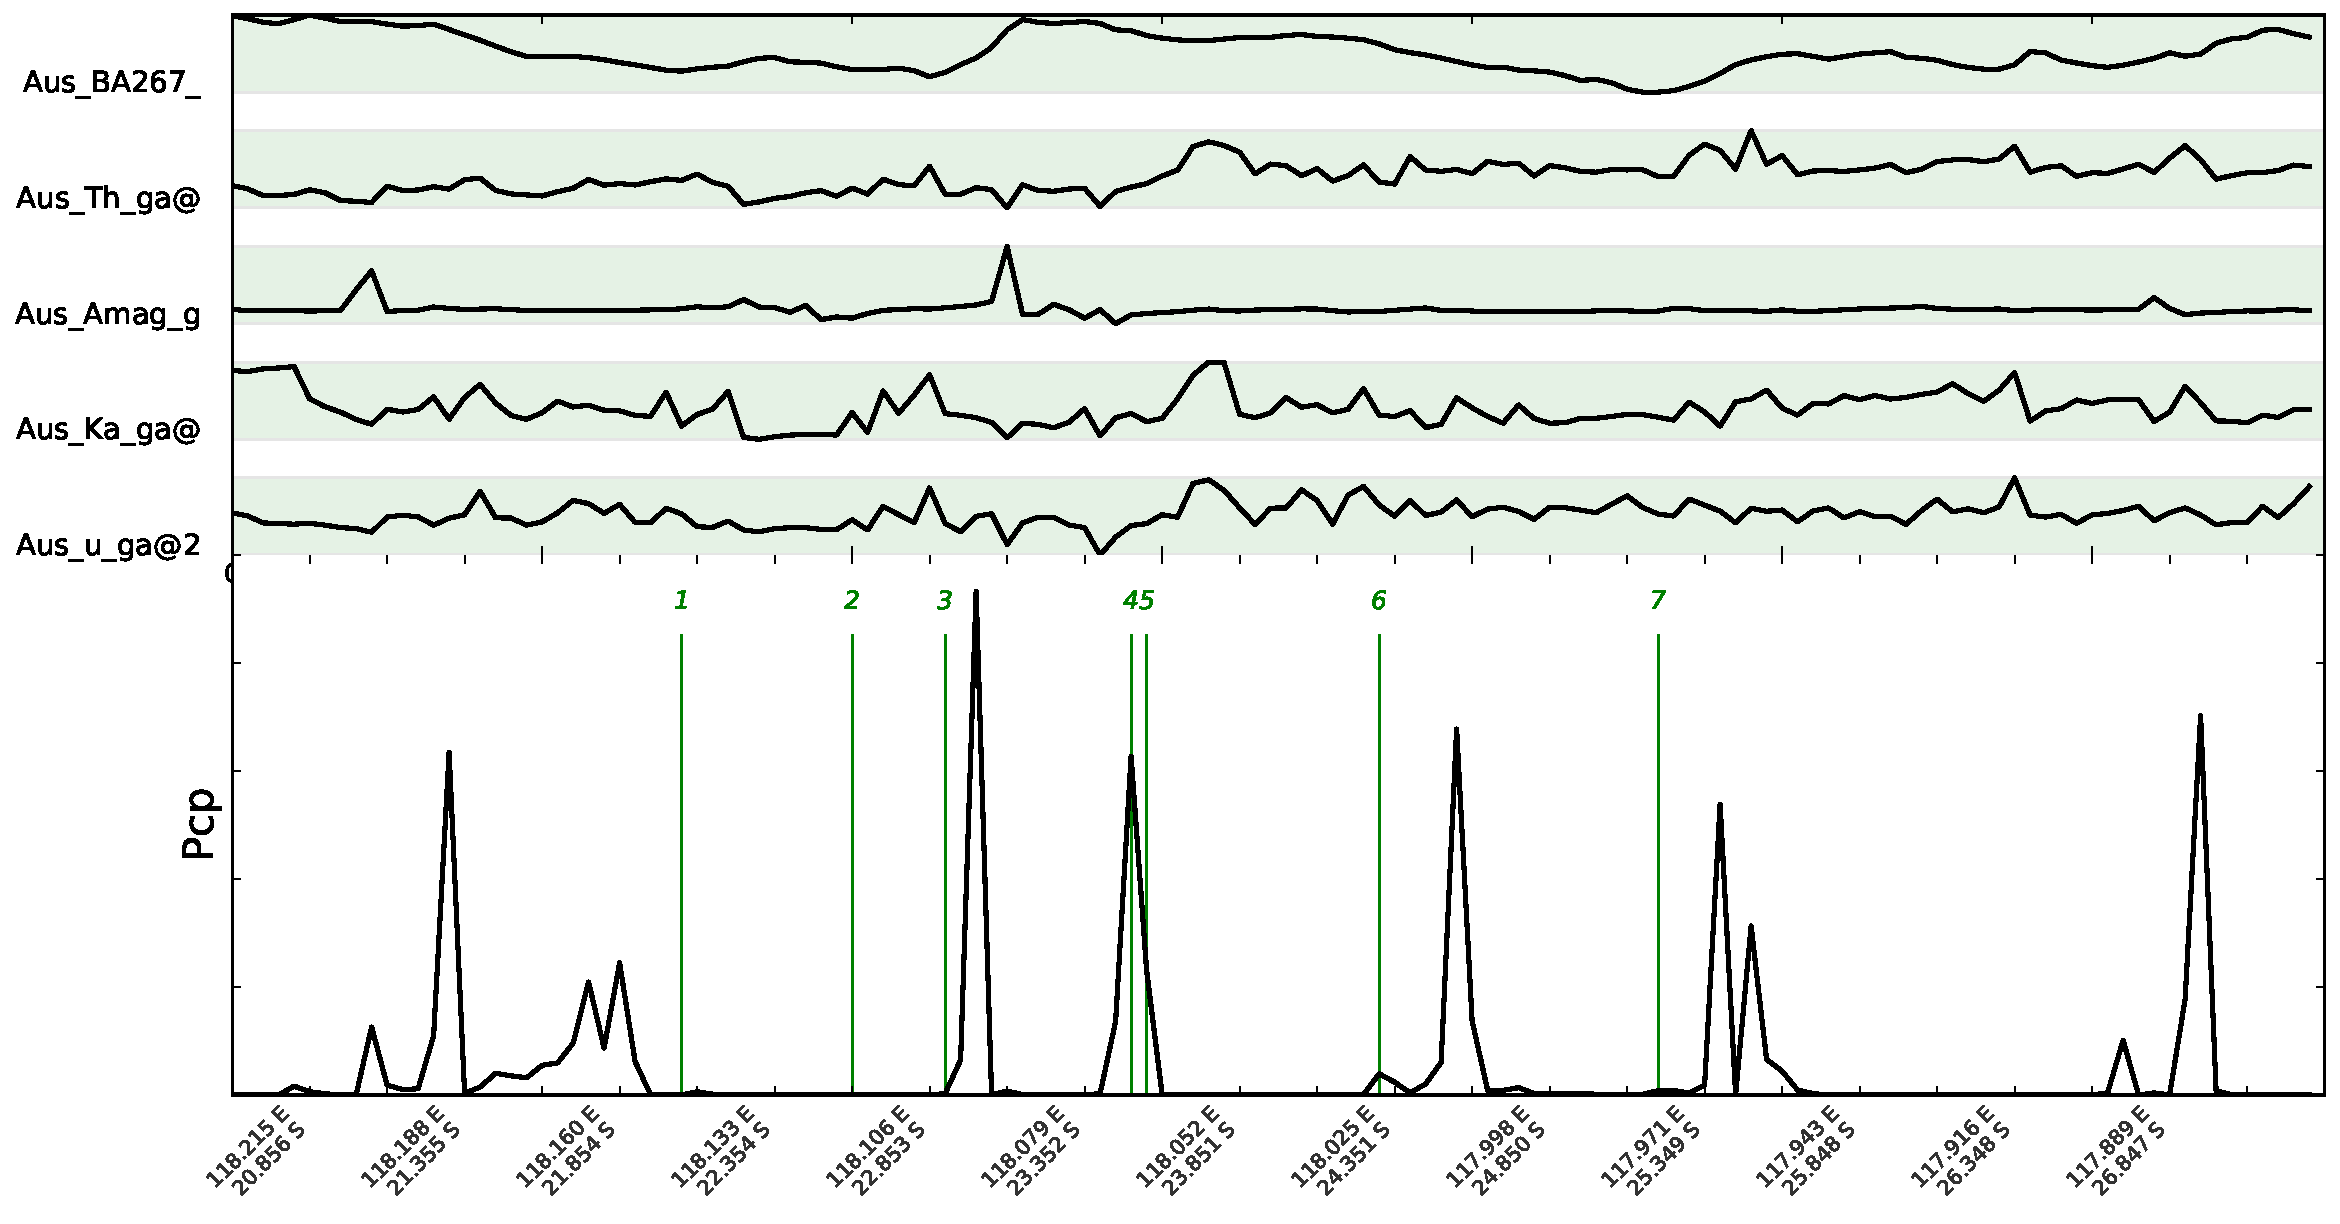
\includegraphics[width=0.9\linewidth]{../fig/ga_vpt_line_12}
		\caption[Line 12]{Line 12 subsampled 1:5 From left: 070 Pilbara Province (Craton/ Block), 1: 041 Hamersley Basin; overlies 070 Pilbara Craton, 2: 070 Pilbara Province (Craton/ Block), 3: 041 Hamersley Basin; overlies 070 Pilbara Craton, 4: 070 Pilbara Province (Craton/ Block), 5: Mount Vernon (100k map) region; 112 Asburton Basin; marginal to Capricorn Orogen, 6: Collier (250k map) region of Capricorn Orogen; southern 035 Gascoyne Province, 7: 093 Yilgarn Craton (Super)-province (Block)
}
		\label{fig:galine12}
	\end{subfigure}
	
	\begin{subfigure}[b]{1\textwidth}
		\centering
		\includegraphics[width=0.9\linewidth]{../fig/ga_vpt_line_12_lo}
		\caption[Line 12]{Line 12 subsampled 1:50 From left: 070 Pilbara Province (Craton/ Block), 1: 041 Hamersley Basin; overlies 070 Pilbara Craton, 2: 070 Pilbara Province (Craton/ Block), 3: 041 Hamersley Basin; overlies 070 Pilbara Craton, 4: 070 Pilbara Province (Craton/ Block), 5: Mount Vernon (100k map) region; 112 Asburton Basin; marginal to Capricorn Orogen, 6: Collier (250k map) region of Capricorn Orogen; southern 035 Gascoyne Province, 7: 093 Yilgarn Craton (Super)-province (Block)
}
		\label{fig:galine12_lo}
	\end{subfigure}
	
	\caption[Line 12]{Line 12}
\end{figure}

\begin{figure}
	\centering
	\begin{subfigure}[b]{1\textwidth}
		\centering
		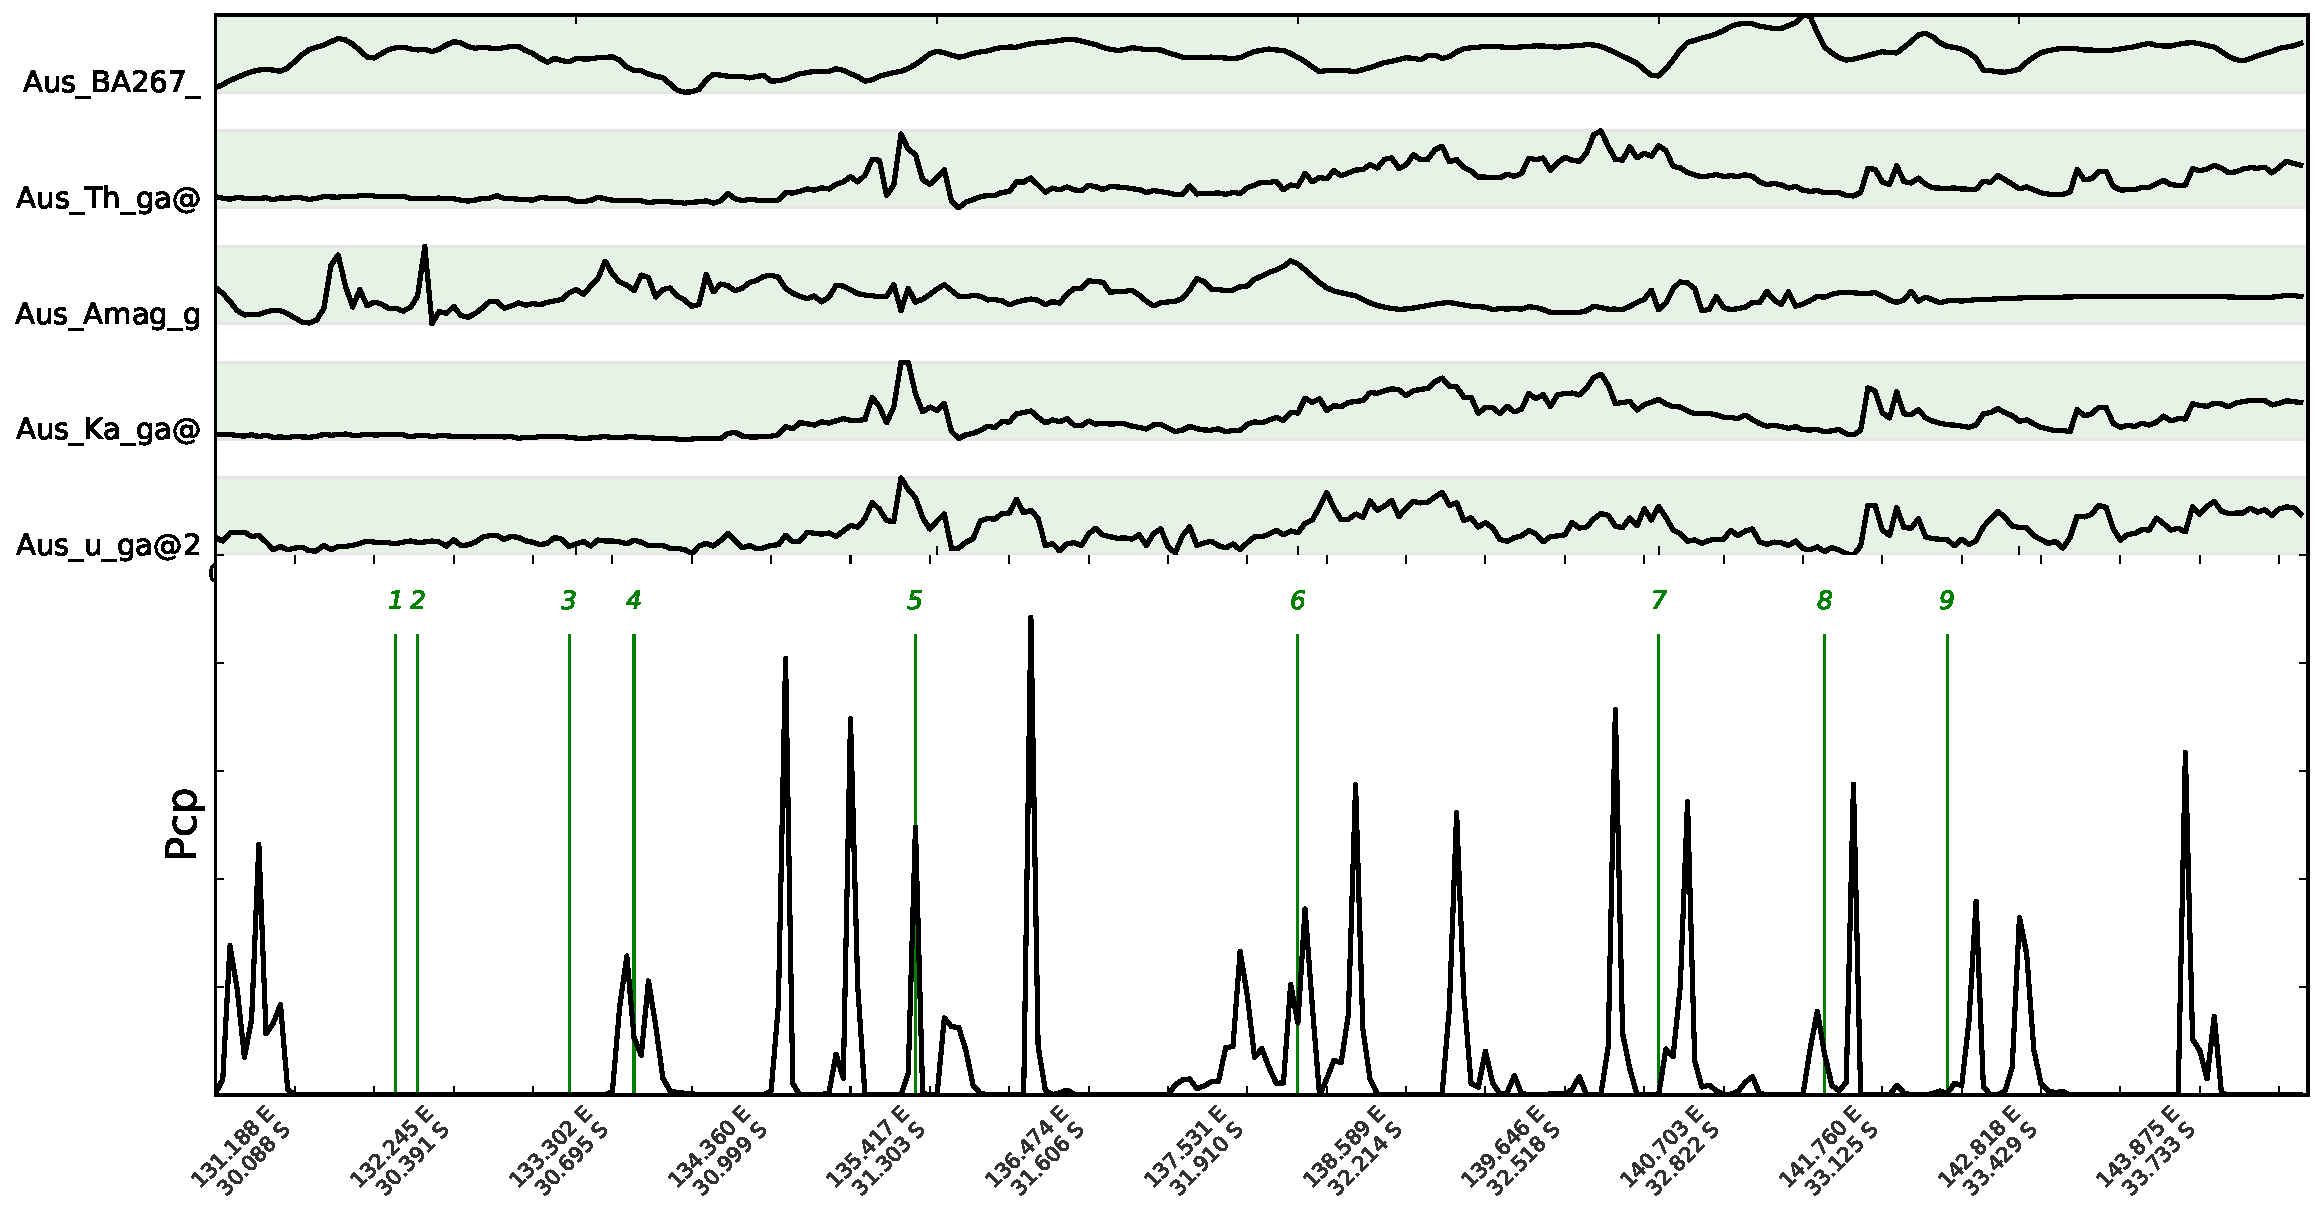
\includegraphics[width=0.9\linewidth]{../fig/ga_vpt_line_14}
		\caption[Line 14]{Line 14 subsampled 1:5 From left: Nawa structural subdomain, basement province (includes Ammaroodina Inlier); in old 036 {superseded} Gawler Craton, 1: Karari Fault Zone; N-margin to 036 Gawler Craton (redefined craton margin), 2: Christie structural subdomain (Barton 250k map); 036 Gawler Craton, 3: Fowler zone (Colona and Coorambie Fault zones), eastern Christie structural subdomain (NW Fowler 250k map); 036 Gawler Craton, 4: Wilgena and Nuyts structural subdomains; 036 Gawler Craton, 5: Gawler Range Volcanic Subprovince (geophysical subdivision); 036 Gawler Craton, 6: 002 Adelaide Province (Fold Belt), 7: 044 Kanmantoo Province (Fold Belt), 8: Glenelg and Stavely Zones; western margin of 047 Lachlan, 9: Western part of 047 Lachlan Province (Fold Belt)
}
		\label{fig:galine14}
	\end{subfigure}
	
	\begin{subfigure}[b]{1\textwidth}
		\centering
		\includegraphics[width=0.9\linewidth]{../fig/ga_vpt_line_14_lo}
		\caption[Line 14]{Line 14 subsampled 1:50 From left: Nawa structural subdomain, basement province (includes Ammaroodina Inlier); in old 036 {superseded} Gawler Craton, 1: Karari Fault Zone; N-margin to 036 Gawler Craton (redefined craton margin), 2: Christie structural subdomain (Barton 250k map); 036 Gawler Craton, 3: Fowler zone (Colona and Coorambie Fault zones), eastern Christie structural subdomain (NW Fowler 250k map); 036 Gawler Craton, 4: Wilgena and Nuyts structural subdomains; 036 Gawler Craton, 5: Gawler Range Volcanic Subprovince (geophysical subdivision); 036 Gawler Craton, 6: 002 Adelaide Province (Fold Belt), 7: 044 Kanmantoo Province (Fold Belt), 8: Glenelg and Stavely Zones; western margin of 047 Lachlan, 9: Western part of 047 Lachlan Province (Fold Belt)
}
		\label{fig:galine14_lo}
	\end{subfigure}
	
	\caption[Line 14]{Line 14}
\end{figure}

\begin{figure}
	\centering
	\begin{subfigure}[b]{1\textwidth}
		\centering
		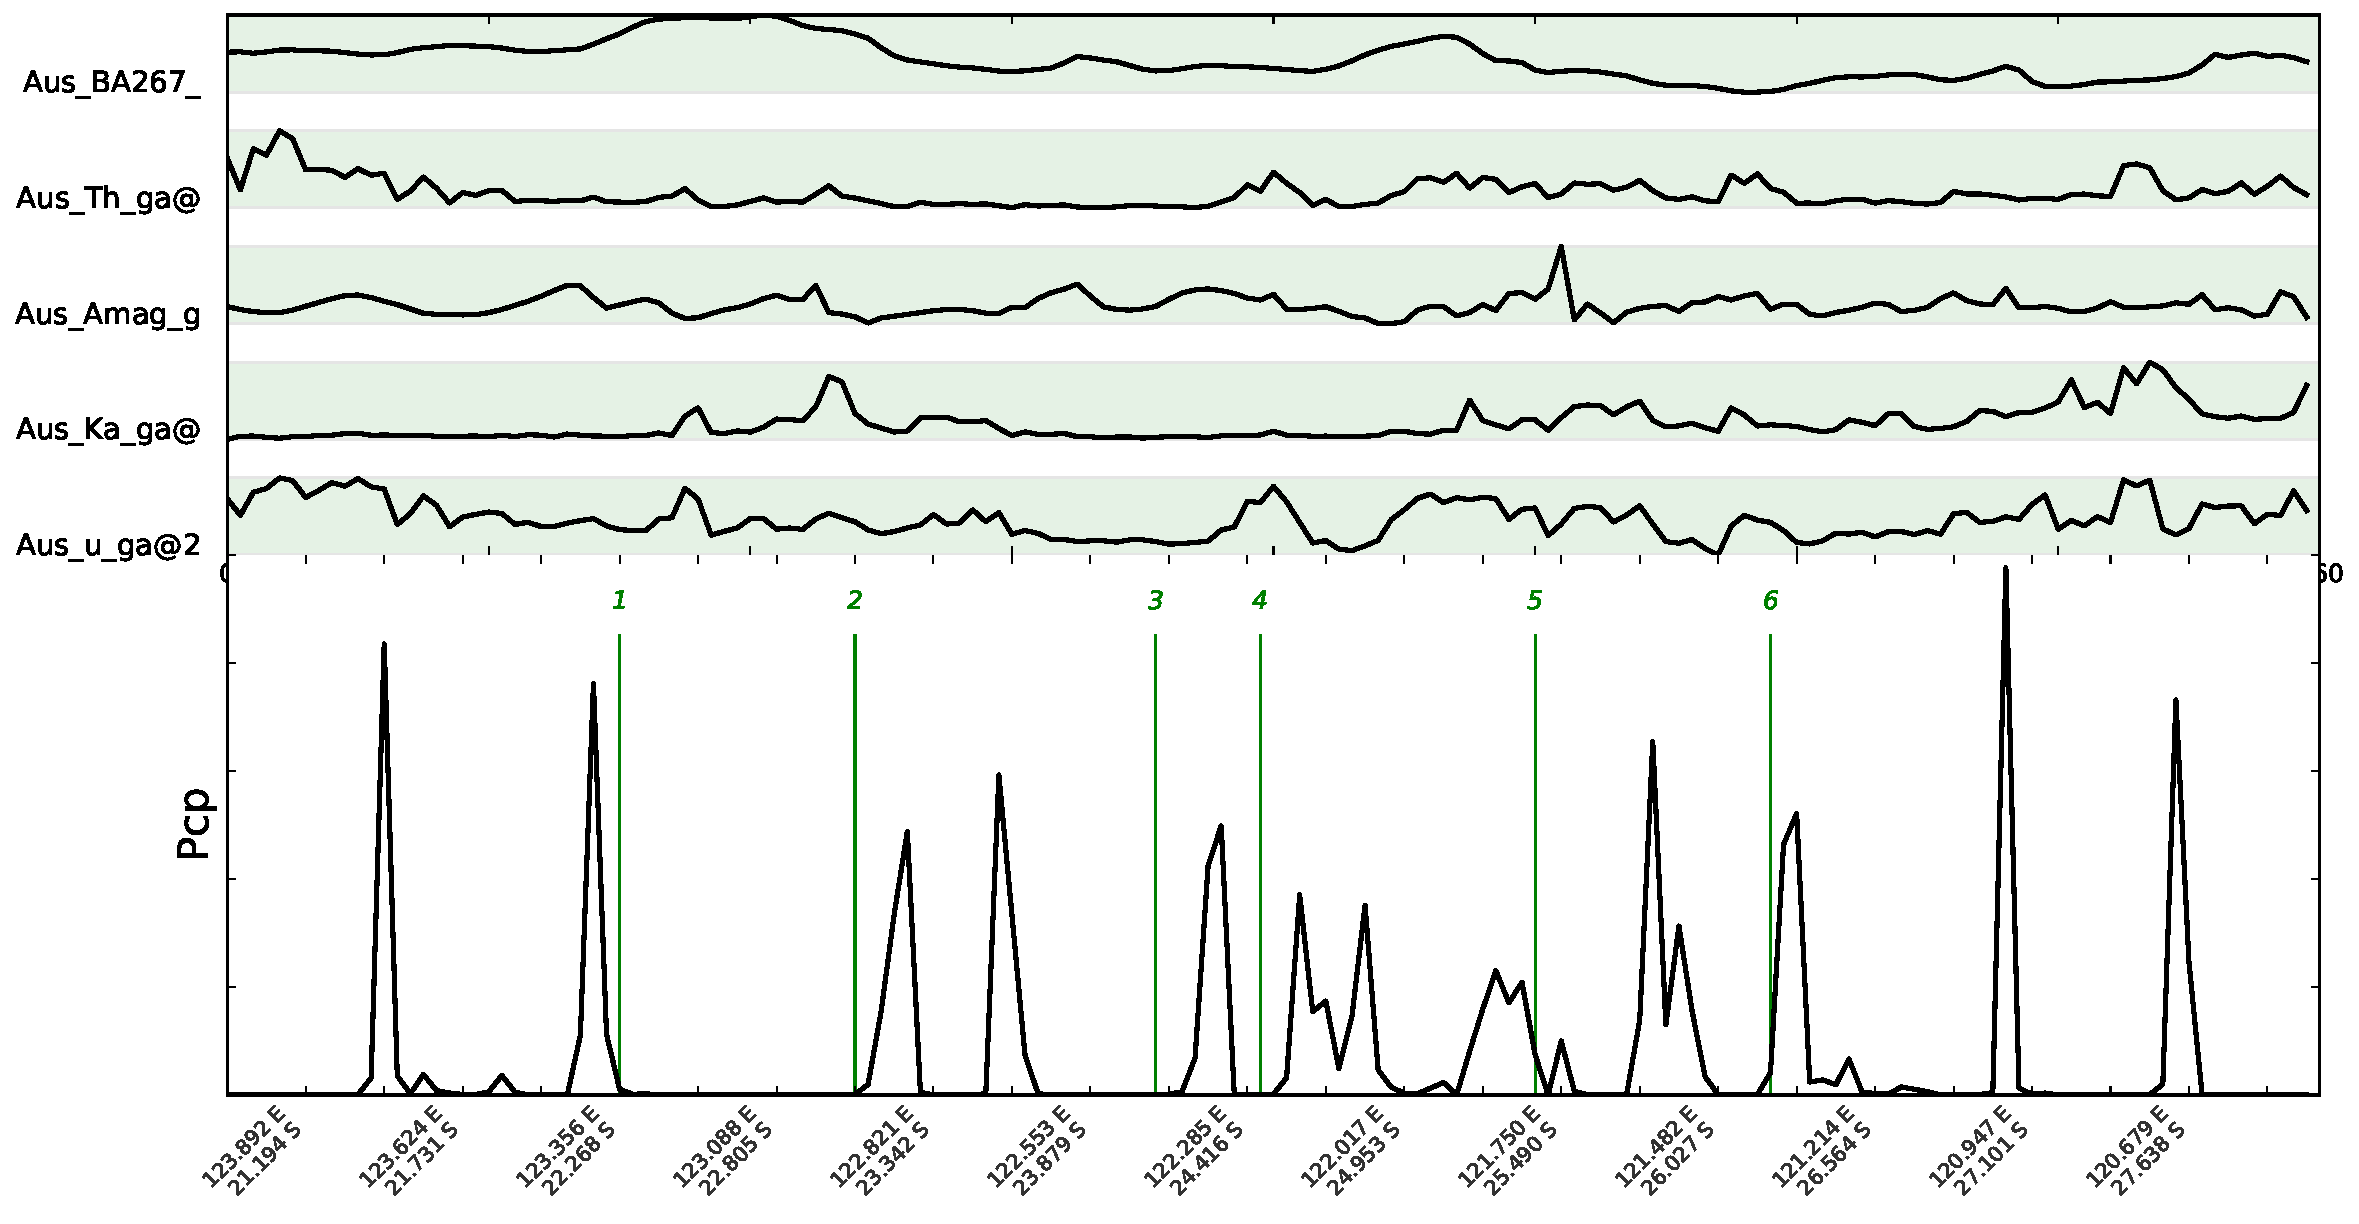
\includegraphics[width=0.9\linewidth]{../fig/ga_vpt_line_15}
		\caption[Line 15]{Line 15 subsampled 1:5 From left: Roeves (gravity feature, Reeves Knoll) region; basement province, 1: Rudall Inlier within  067 Paterson Province, 2: LD Lake Dissapointment  region (Gunanya 1:250k map); 067 Paterson Province (?), 3: Capricorn East (geophysical) region of Capricorn Orogen (e.g., Trainor 100k map); basement province (poorly defined), 4: Basement to 011 Bangemall Basin; Capricorn Orogen, 5: Overlies NE Yilgarn, 6: 093 Yilgarn Craton (Super)-province (Block)
}
		\label{fig:galine15}
	\end{subfigure}
	
	\begin{subfigure}[b]{1\textwidth}
		\centering
		\includegraphics[width=0.9\linewidth]{../fig/ga_vpt_line_15_lo}
		\caption[Line 15]{Line 15 subsampled 1:50 From left: Roeves (gravity feature, Reeves Knoll) region; basement province, 1: Rudall Inlier within  067 Paterson Province, 2: LD Lake Dissapointment  region (Gunanya 1:250k map); 067 Paterson Province (?), 3: Capricorn East (geophysical) region of Capricorn Orogen (e.g., Trainor 100k map); basement province (poorly defined), 4: Basement to 011 Bangemall Basin; Capricorn Orogen, 5: Overlies NE Yilgarn, 6: 093 Yilgarn Craton (Super)-province (Block)
}
		\label{fig:galine15_lo}
	\end{subfigure}
	
	\caption[Line 15]{Line 15}
\end{figure}

\begin{figure}
	\centering
	\begin{subfigure}[b]{1\textwidth}
	\centering
	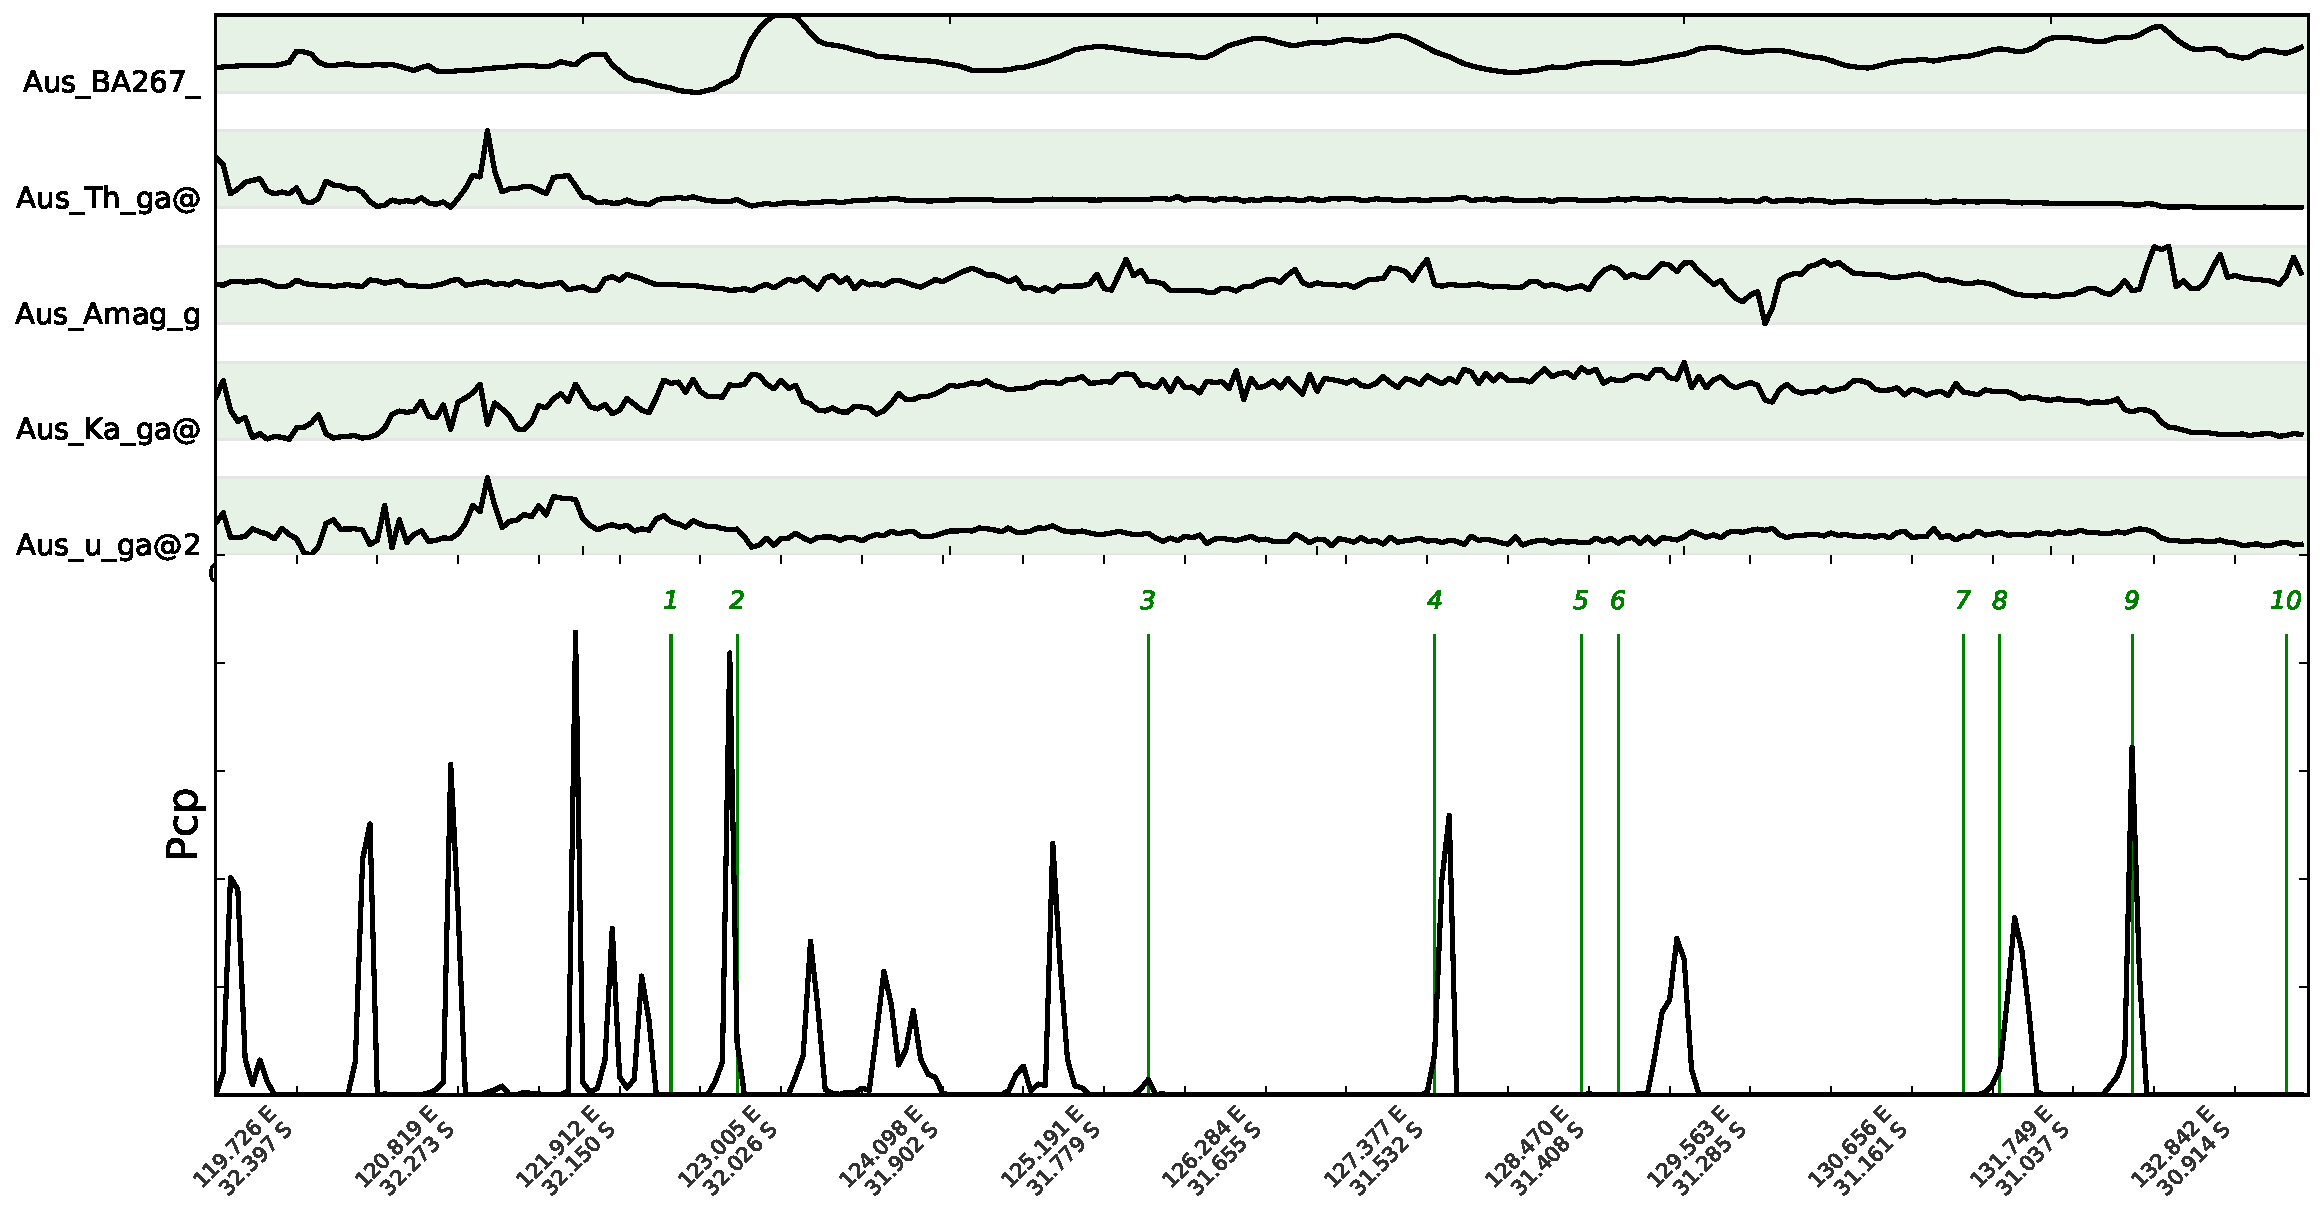
\includegraphics[width=0.9\linewidth]{../fig/ga_vpt_line_16}
	\caption[Line 16]{Line 15 subsampled 1:5 From left: 093 Yilgarn Craton (Super)-province (Block), 1: Mulga Rock (overprinted geophysical) zone; 093 Yilgarn (Super) province, 2: 003 Albany-Fraser Province, 3: Madura (250k map) region (or Naretha region); basement province, 4: Forrest (250k map) region, basement province, 5: Waigen (250k map) region; basement province, 6: Coompana Province (Block); basement province, 7: Cook (geophysically overprinted) zone (e.g., Cook 100k map); dolerite dyke swarm at northern edge of Coompana Block, basement unit (WT: Watson zone in version-1 map), 8: Christie structural subdomain (Barton 250k map); 036 Gawler Craton, 9: Fowler zone (Colona and Coorambie Fault zones), eastern Christie structural subdomain (NW Fowler 250k map); 036 Gawler Craton, 10: Wilgena and Nuyts structural subdomains; 036 Gawler Craton
}
	\label{fig:galine16}
	\end{subfigure}
	
	\begin{subfigure}[b]{1\textwidth}
	\centering
	\includegraphics[width=0.9\linewidth]{../fig/ga_vpt_line_16_lo}
	\caption[Line 16]{Line 16 subsampled 1:50 From left: 093 Yilgarn Craton (Super)-province (Block), 1: Mulga Rock (overprinted geophysical) zone; 093 Yilgarn (Super) province, 2: 003 Albany-Fraser Province, 3: Madura (250k map) region (or Naretha region); basement province, 4: Forrest (250k map) region, basement province, 5: Waigen (250k map) region; basement province, 6: Coompana Province (Block); basement province, 7: Cook (geophysically overprinted) zone (e.g., Cook 100k map); dolerite dyke swarm at northern edge of Coompana Block, basement unit (WT: Watson zone in version-1 map), 8: Christie structural subdomain (Barton 250k map); 036 Gawler Craton, 9: Fowler zone (Colona and Coorambie Fault zones), eastern Christie structural subdomain (NW Fowler 250k map); 036 Gawler Craton, 10: Wilgena and Nuyts structural subdomains; 036 Gawler Craton
}
	\label{fig:galine16_lo}
	\end{subfigure}
	
	\caption[Line 16]{Line 16}
\end{figure}

\begin{figure}
	\centering
	\begin{subfigure}[b]{1\textwidth}
		\centering
		\includegraphics[width=0.65\linewidth]{../fig/no_radio_ga_vpt_line_2}
		\caption[Line 2, no radometry]{Line 2 without radiometric data. Subsampled 1:5 From left: Oscar Range region, basement province, 1: Nookanbah (250k) region, basement province, 2: Basement to Barbwire Terrace of 017 Canning Basin, 3: Lagrange (250k map) region, basement province, 4: Koop 100k map region (geophysicallly overprinted zone); basement province, 5: Roeves (gravity feature, Reeves Knoll) region; basement province, 6: 067 Paterson Province, 7: Rudall Inlier within  067 Paterson Province, 8: LD Lake Dissapointment  region (Gunanya 1:250k map); 067 Paterson Province (?), 9: Capricorn East (geophysical) region of Capricorn Orogen (e.g., Trainor 100k map); basement province (poorly defined), 10: Basement to 011 Bangemall Basin; Capricorn Orogen, 11: Overlies NE Yilgarn, 12: 093 Yilgarn Craton (Super)-province (Block)
}
	\label{fig:galine2_no}
\end{subfigure}
	
	\begin{subfigure}[b]{1\textwidth}
		\centering
		\includegraphics[width=0.65\linewidth]{../fig/no_radio_ga_vpt_line_12}
		\caption[Line 12, no radometry]{Line 12 without radiometric data. Subsampled 1:5. From left: 070 Pilbara Province (Craton/ Block), 1: 041 Hamersley Basin; overlies 070 Pilbara Craton, 2: 070 Pilbara Province (Craton/ Block), 3: 041 Hamersley Basin; overlies 070 Pilbara Craton, 4: 070 Pilbara Province (Craton/ Block), 5: Mount Vernon (100k map) region; 112 Asburton Basin; marginal to Capricorn Orogen, 6: Collier (250k map) region of Capricorn Orogen; southern 035 Gascoyne Province, 7: 093 Yilgarn Craton (Super)-province (Block)
}
	\label{fig:galine12_no}
\end{subfigure}
	
	\begin{subfigure}[b]{1\textwidth}
			\centering
			\includegraphics[width=0.65\linewidth]{../fig/no_radio_ga_vpt_line_15}
			\caption[Line 15, no radometry]{Line 15 without radiometric data. Subsampled 1:5. From left: Roeves (gravity feature, Reeves Knoll) region; basement province, 1: Rudall Inlier within  067 Paterson Province, 2: LD Lake Dissapointment  region (Gunanya 1:250k map); 067 Paterson Province (?), 3: Capricorn East (geophysical) region of Capricorn Orogen (e.g., Trainor 100k map); basement province (poorly defined), 4: Basement to 011 Bangemall Basin; Capricorn Orogen, 5: Overlies NE Yilgarn, 6: 093 Yilgarn Craton (Super)-province (Block)
}
			\label{fig:galine15_no}
\end{subfigure}
		
	\caption[Line 2, 12 and 15 without radometry]{Lines 2, 12 and 15. Off-line changepoint detection without use of radiometric data. Sub-sampled 1:5.}
\end{figure}

\begin{figure}
	\centering
	\begin{subfigure}[b]{1\textwidth}
		\centering
		\includegraphics[width=0.7\linewidth]{../fig/no_radio_ga_vpt_line_13}
		\caption[Line 13, no radometry]{Line 13 without radiometric data. Subsampled 1:5. From left: Waigen (250k map) region; basement province, 1: Nawa structural subdomain, basement province (includes Ammaroodina Inlier); in old 036 {superseded} Gawler Craton, 2: Western magnetic part of Mabel Creek (100k map) region (geophysical subdivision); in old 036 (superseded) Gawler Craton, 3: Karari Fault Zone; N-margin to 036 Gawler Craton (redefined craton margin), 4: Christie structural subdomain (Barton 250k map); 036 Gawler Craton, 5: Challenger (Mine) region (Coober Pedy 250k map); 036 Gawler Craton, 6: Fowler zone (Colona and Coorambie Fault zones), eastern Christie structural subdomain (NW Fowler 250k map); 036 Gawler Craton, 7: Wilgena and Nuyts structural subdomains; 036 Gawler Craton, 8: Gawler Range Volcanic Subprovince (geophysical subdivision); 036 Gawler Craton, 9: 002 Adelaide Province (Fold Belt), 10: Curnamona craton (nucleus), basement province (includes Benagerie Ridge), 11: 108 Willyama subprovince (Block) and Olary subprovince (Willyama Inliers in South Australia) adjoining southern Curnamona (geological) craton (nucleus); 016 Broken Hill Province (Block), 12: Covered Willyama Province; 016 Broken Hill Block, 13: 108 Willyama subprovince (Block) and Olary subprovince (Willyama Inliers in South Australia) adjoining southern Curnamona (geological) craton (nucleus); 016 Broken Hill Province (Block), 14: Redan (geophysical overprinting) Zone; southern margin of 016 Broken Hill Province (Block), 15: 044 Kanmantoo Province (Fold Belt), 16: Glenelg and Stavely Zones; western margin of 047 Lachlan, 17: Western part of 047 Lachlan Province (Fold Belt)
}
	\label{fig:galine13_no}
\end{subfigure}

\begin{subfigure}[b]{1\textwidth}
	\centering
	\includegraphics[width=0.7\linewidth]{../fig/no_radio_ga_vpt_line_14}
	\caption[Line 14, without radiometry]{Line 14 without radiometric data. Sub-sampled 1:5. From left: Nawa structural subdomain, basement province (includes Ammaroodina Inlier); in old 036 {superseded} Gawler Craton, 1: Karari Fault Zone; N-margin to 036 Gawler Craton (redefined craton margin), 2: Christie structural subdomain (Barton 250k map); 036 Gawler Craton, 3: Fowler zone (Colona and Coorambie Fault zones), eastern Christie structural subdomain (NW Fowler 250k map); 036 Gawler Craton, 4: Wilgena and Nuyts structural subdomains; 036 Gawler Craton, 5: Gawler Range Volcanic Subprovince (geophysical subdivision); 036 Gawler Craton, 6: 002 Adelaide Province (Fold Belt), 7: 044 Kanmantoo Province (Fold Belt), 8: Glenelg and Stavely Zones; western margin of 047 Lachlan, 9: Western part of 047 Lachlan Province (Fold Belt)
}
\label{fig:galine14_no}
\end{subfigure}

\caption[Line 13 and 14 without radiometry]{Lines 13 and 14. Off-line changepoint detection without use of radiometric data. Sub-sampled 1:5.}
\end{figure}

\begin{figure}
	\centering
	\begin{subfigure}[b]{1\textwidth}
		\centering
		\includegraphics[width=0.7\linewidth]{../fig/no_radio_ga_vpt_line_16}
		\caption[Line 16, no radiometry]{Line 16 without radiometric data. Sub-sampled 1:5.} 
		\label{fig:galine16_no}
	\end{subfigure}
	
	\begin{subfigure}[b]{1\textwidth}
		\centering
		\includegraphics[width=0.7\linewidth]{../fig/no_radio_ga_vpt_line_16_lo}
		\caption[Line 16, no radiometry, subsampled 50]{Line 16 without radiometric data. Sub-sampled 1:50.}
		\label{fig:galine16_no_lo}
	\end{subfigure}
	
	
	\caption[Line 16 without radiometry. Sub-sampled 1:5 and 1:50.]{Lines 16, sub-sampled 1:5 and 16 sub-sampled 1:50. Off-line changepoint detection without use of radiometric data. Sub-sampled 1:5. From left: 093 Yilgarn Craton (Super)-province (Block), 1: Mulga Rock (overprinted geophysical) zone; 093 Yilgarn (Super) province, 2: 003 Albany-Fraser Province, 3: Madura (250k map) region (or Naretha region); basement province, 4: Forrest (250k map) region, basement province, 5: Waigen (250k map) region; basement province, 6: Coompana Province (Block); basement province, 7: Cook (geophysically overprinted) zone (e.g., Cook 100k map); dolerite dyke swarm at northern edge of Coompana Block, basement unit (WT: Watson zone in version-1 map), 8: Christie structural subdomain (Barton 250k map); 036 Gawler Craton, 9: Fowler zone (Colona and Coorambie Fault zones), eastern Christie structural subdomain (NW Fowler 250k map); 036 Gawler Craton, 10: Wilgena and Nuyts structural subdomains; 036 Gawler Craton
}
\end{figure}

	\begin{figure}
		\centering
		\begin{subfigure}[b]{1\textwidth}
			\centering
			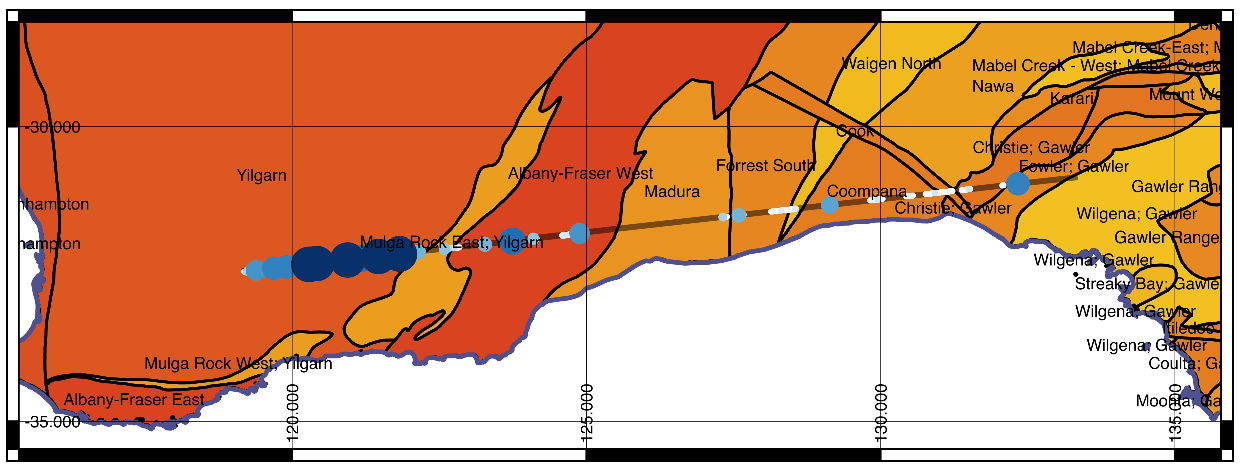
\includegraphics[width=0.78\linewidth]{../fig/maps/Line_16_S5_T100}
			\caption{}
			\label{fig:Ng1} 
		\end{subfigure}

		\begin{subfigure}[b]{1\textwidth}
			\centering
			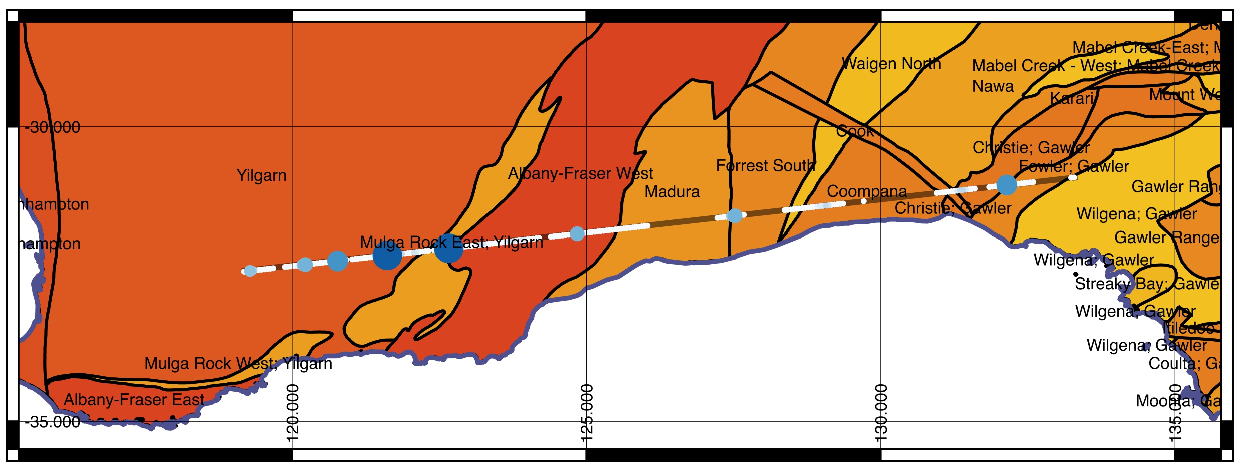
\includegraphics[width=0.78\linewidth]{../fig/maps/Line_16_S50_T100}
			\caption{}
			\label{fig:Ng2}
		\end{subfigure}

		
		\begin{subfigure}[b]{1\textwidth}
			\centering
			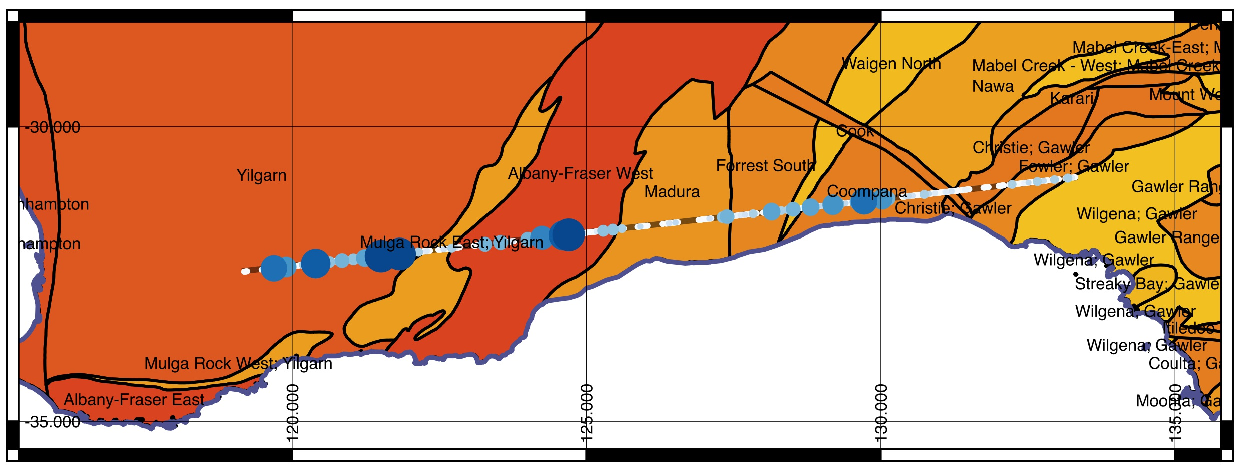
\includegraphics[width=0.78\linewidth]{../fig/maps/Line_16_S5_T100_No_Radio}
			\caption{}
			\label{fig:Ng3}
		\end{subfigure}
		
		\begin{subfigure}[b]{1\textwidth}
			\centering
			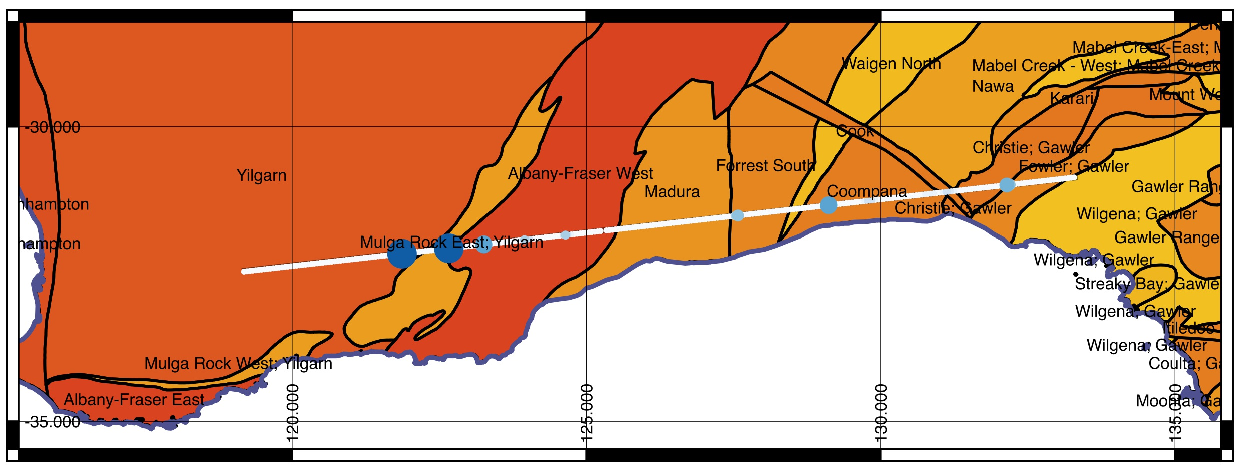
\includegraphics[width=0.78\linewidth]{../fig/maps/Line_16_S50_T100_No_Radio}
			\caption{}
			\label{fig:Ng4}
		\end{subfigure}		
		

		\caption[Resampling and radiometry compararasion for Line 16]{Line 16 (a) Sub-sampled 1:5, all parameters (b) Sub-sampled 1:50. (c) No radiometric data, sub-sampled 1:5 (d) No radiometric data sub-sampled 1:50. The dots symbolise probability (Pcp), darker. Smallest white is $10^-6$ and largest dark blue is $1$. See plots for exact values. }
	\end{figure}


\begin{sidewaysfigure}
	\centering


\centering
\includegraphics[width=1\linewidth]{"../fig/maps/All lines"}
\caption[Change points for all lines]{Lines subsampled 1:5. Changepoints calculated from gravity, magnetic and radiometric (K, Th and U).}
\label{fig:all-lines}

\end{sidewaysfigure}


\begin{sidewaysfigure}
	\centering
	
	
	\centering
	\includegraphics[width=1\linewidth]{"../fig/maps/slope_of_slope"}
	\caption[Derivate of changes in magnetic potential field.]{This map shows the derivative of changes in the magnetic potential field. Gawler, Musgrave and Yilgarn is well recognizable. This is an example of tests of 2D datasets to guide interpolation of change-points. Moreover, the steep second order derivatives relates to the background noise or spikiness in the change-point detection for catatonic areas with short sample length.}
	\label{fig:slopes}
	
\end{sidewaysfigure}


\begin{sidewaysfigure}
	\centering
	
	\centering
	\includegraphics[width=1\linewidth]{"../fig/maps/rough_change"}
	\caption[Derivate of changes in magnetic potential field and suggested changepoints.]{Roughness and detected change-points.}
	\label{fig:slopes_and_change}
	
\end{sidewaysfigure}


%
%
\printbibliography
\end{document}